\section{\ac{SMT}-solvers}

\subsection{School-level system of equations}

I've got this school-level system of equations copypasted from Wikipedia
\footnote{\url{https://en.wikipedia.org/wiki/System_of_linear_equations}}:

\begin{alignat*}{7}
3x &&\; + \;&& 2y             &&\; - \;&& z  &&\; = \;&& 1 & \\
2x &&\; - \;&& 2y             &&\; + \;&& 4z &&\; = \;&& -2 & \\
-x &&\; + \;&& \tfrac{1}{2} y &&\; - \;&& z  &&\; = \;&& 0 &
\end{alignat*}

Will it be possible to solve it using Z3? Here it is:

\begin{lstlisting}
#!/usr/bin/python
from z3 import *

x = Real('x')
y = Real('y')
z = Real('z')
s = Solver()
s.add(3*x + 2*y - z == 1)
s.add(2*x - 2*y + 4*z == -2)
s.add(-x + 0.5*y - z == 0)
print s.check()
print s.model()
\end{lstlisting}

We see this after run:

\begin{lstlisting}
sat
[z = -2, y = -2, x = 1]
\end{lstlisting}

If we change any equation in some way so it will have no solution, s.check() will return ``unsat''.

I've used ``Real'' \textit{sort} (some kind of data type in \ac{SMT}-solvers)
because the last expression equals to $\frac{1}{2}$, which is, of course, a real number.
For the integer system of equations, ``Int'' \textit{sort} would work fine.

Python (and other high-level \ac{PL}s like C\#) interface is highly popular, because it's practical, but in fact, 
there is a standard language for \ac{SMT}-solvers called SMT-LIB
\footnote{\url{http://smtlib.cs.uiowa.edu/papers/smt-lib-reference-v2.5-r2015-06-28.pdf}}.

Our example rewritten to it looks like this:

\begin{lstlisting}
(declare-const x Real)
(declare-const y Real)
(declare-const z Real)
(assert (=(-(+(* 3 x) (* 2 y)) z) 1))
(assert (=(+(-(* 2 x) (* 2 y)) (* 4 z)) -2))
(assert (=(-(+ (- 0 x) (* 0.5 y)) z) 0))
(check-sat)
(get-model)
\end{lstlisting}

This language is very close to LISP, but is somewhat hard to read for untrained eyes.

Now we run it:

\begin{lstlisting}
% z3 -smt2 example.smt
sat
(model
  (define-fun z () Real
    (- 2.0))
  (define-fun y () Real
    (- 2.0))
  (define-fun x () Real
    1.0)
)
\end{lstlisting}

So when you look back to my Python code, you may feel that these 3 expressions could be executed.
This is not true: Z3Py API offers overloaded operators, so expressions are constructed and passed into the guts of Z3 without any execution
\footnote{\url{https://github.com/Z3Prover/z3/blob/6e852762baf568af2aad1e35019fdf41189e4e12/src/api/python/z3.py}}.
I would call it ``embedded \ac{DSL}''.

Same thing for Z3 C++ API, you may find there ``operator+'' declarations and many more
\footnote{\url{https://github.com/Z3Prover/z3/blob/6e852762baf568af2aad1e35019fdf41189e4e12/src/api/c\%2B\%2B/z3\%2B\%2B.h}}.

Z3 \ac{API}s for Java, ML and .NET are also exist
\footnote{\url{https://github.com/Z3Prover/z3/tree/6e852762baf568af2aad1e35019fdf41189e4e12/src/api}}.\\
\\
Z3Py tutorial: \url{https://github.com/ericpony/z3py-tutorial}.

Z3 tutorial which uses SMT-LIB language: \url{http://rise4fun.com/Z3/tutorial/guide}.

\subsection{Another school-level system of equations}
\label{eq2_SMT}

I've found this somewhere at Facebook:

\begin{figure}[H]
\centering
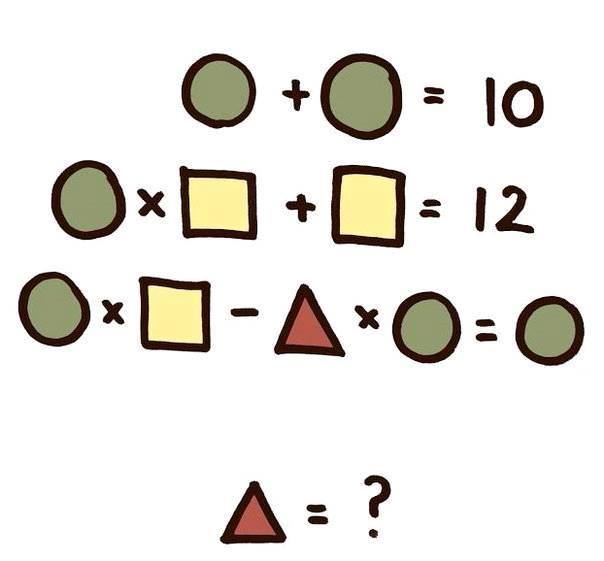
\includegraphics[scale=0.3]{SMT/equation.jpg}
\caption{System of equations}
\end{figure}

It's that easy to solve it in Z3:

\begin{lstlisting}
#!/usr/bin/python
from z3 import *

circle, square, triangle = Ints('circle square triangle')
s = Solver()
s.add(circle+circle==10)
s.add(circle*square+square==12)
s.add(circle*square-triangle*circle==circle)
print s.check()
print s.model()
\end{lstlisting}

\begin{lstlisting}
sat
[triangle = 1, square = 2, circle = 5]
\end{lstlisting}

\subsection{Connection between \ac{SAT} and \ac{SMT} solvers}

\ac{SMT}-solvers are frontends to \ac{SAT} solvers, i.e.,
they translating input SMT expressions into \ac{CNF} and feed SAT-solver with it.
Translation process is sometimes called ``bit blasting''.
Some \ac{SMT}-solvers uses external SAT-solver: STP uses MiniSAT or CryptoMiniSAT as backend.
Some other \ac{SMT}-solvers (like Z3) has their own SAT solver.

% subsections
\subsection{De Bruijn sequences; leading/trailing zero bits counting}

\subsubsection{Introduction}

Let's imagine there is a very simplified code lock accepting 2 digits, but it has no "enter" key, it just checks 2 last entered digits.
Our task is to brute force each 2-digit combination.
Naïve method is to try 00, 01, 02 ... 99.
That require 2*100=200 key pressings.
Will it be possible to reduce number of key pressings during brute-force?
It is indeed so, with the help of De Bruijn sequences.
We can generate them for the code lock, using Wolfram Mathematica:

\begin{lstlisting}
In[]:= DeBruijnSequence[{0, 1, 2, 3, 4, 5, 6, 7, 8, 9}, 2]
Out[]= {6, 8, 6, 5, 4, 3, 2, 1, 7, 8, 7, 1, 1, 0, 9, 0, 8, 0, 6, 6, \
0, 5, 5, 0, 4, 4, 0, 3, 3, 0, 2, 7, 2, 2, 0, 7, 7, 9, 8, 8, 9, 9, 7, \
0, 0, 1, 9, 1, 8, 1, 6, 1, 5, 1, 4, 1, 3, 7, 3, 1, 2, 9, 2, 8, 2, 6, \
2, 5, 2, 4, 7, 4, 2, 3, 9, 3, 8, 3, 6, 3, 5, 7, 5, 3, 4, 9, 4, 8, 4, \
6, 7, 6, 4, 5, 9, 5, 8, 5, 6, 9}
\end{lstlisting}

The result has exactly 100 digits, which is 2 times less than our initial idea can offer.
By scanning visually this 100-digits array, you'll find any number in 00..99 range.
All numbers are overlapped with each other: second half of each number is also first half of the next number, etc.

Here is another. We need a sequence of binary bits with all 3-bit numbers in it:

\begin{lstlisting}
In[]:= DeBruijnSequence[{0, 1}, 3]
Out[]= {1, 0, 1, 0, 0, 0, 1, 1}
\end{lstlisting}

Sequence length is just 8 bits, but it has all binary numbers in 000..111 range.
You may visually spot 000 in the middle of sequence.
111 is also present: two first bits of it at the end of sequence and the last bit is in the beginning.
This is so because De Bruijn sequences are cyclic.

There is also visual demonstration: \url{http://demonstrations.wolfram.com/DeBruijnSequences/}.

\subsubsection{Trailing zero bits counting}

In \href{https://en.wikipedia.org/wiki/De_Bruijn_sequence}{the Wikipedia article about De Bruijn sequences} we can find:

\begin{framed}
\begin{quotation}
The symbols of a De Bruijn sequence written around a circular object (such as a wheel of a robot) can be used to identify its angle by examining the n consecutive symbols facing a fixed point.
\end{quotation}
\end{framed}

Indeed: if we know De Bruijn sequence and we observe only part of it (any part), we can deduce exact position of this part within sequence.

Let's see, how this feature can be used.

Let's say, there is a need to detect position of input bit within 32-bit word.
For 0x1, the algorithm should report 1.
2 for 0x2.
3 for 0x4.
And 31 for 0x80000000.

The result is in 0..31 range, so the result can be stored in 5 bits.

We can construct binary De Bruijn sequence for all 5-bit numbers:

\begin{lstlisting}
In[]:= tmp = DeBruijnSequence[{0, 1}, 5]
Out[]= {1, 1, 1, 0, 0, 1, 1, 0, 1, 0, 1, 1, 1, 1, 1, 0, 1, 1, 0, 0, 0, 1, 0, 1, 0, 0, 1, 0, 0, 0, 0, 0}

In[]:= BaseForm[FromDigits[tmp, 2], 16]
Out[]:= e6bec520
\end{lstlisting}

Let's also recall that division some number by $2^n$ number is the same thing as shifting it by $n$ bits.
So if you divide 0xe6bec520 by 1, the result is not shifted, it is still the same.
If if divide 0xe6bec520 by 4 ($2^2$), the result is shifted by 2 bits.
We then take result and isolate lowest 5 bits.
This result is unique number for each input.
Let's shift 0xe6bec520 by all possible count number, and we'll get all possible last 5-bit values:

\begin{lstlisting}
In[]:= Table[BitAnd[BitShiftRight[FromDigits[tmp, 2], i], 31], {i, 0, 31}]
Out[]= {0, 16, 8, 4, 18, 9, 20, 10, 5, 2, 17, 24, 12, 22, 27, 29, \
30, 31, 15, 23, 11, 21, 26, 13, 6, 19, 25, 28, 14, 7, 3, 1}
\end{lstlisting}

The table has no duplicates:

\begin{lstlisting}
In[]:= DuplicateFreeQ[%]
Out[]= True
\end{lstlisting}

Using this table, it's easy to build a \textit{magic} table.
OK, now working C example:

\begin{lstlisting}[style=customc]
#include <stdint.h>
#include <stdio.h>

int magic_tbl[32];

// returns single bit position counting from LSB
// not working for i==0
int bitpos (uint32_t i)
{
	return magic_tbl[(0xe6bec520/i) & 0x1F];
};

int main()
{
	// construct magic table
	// may be omitted in production code
	for (int i=0; i<32; i++)
		magic_tbl[(0xe6bec520/(1<<i)) & 0x1F]=i;

	// test
	for (int i=0; i<32; i++)
	{
		printf ("input=0x%x, result=%d\n", 1<<i, bitpos (1<<i));
	};
};
\end{lstlisting}

Here we feed our bitpos() function with numbers in 0..0x80000000 range and we got:

\begin{lstlisting}
input=0x1, result=0
input=0x2, result=1
input=0x4, result=2
input=0x8, result=3
input=0x10, result=4
input=0x20, result=5
input=0x40, result=6
input=0x80, result=7
input=0x100, result=8
input=0x200, result=9
input=0x400, result=10
input=0x800, result=11
input=0x1000, result=12
input=0x2000, result=13
input=0x4000, result=14
input=0x8000, result=15
input=0x10000, result=16
input=0x20000, result=17
input=0x40000, result=18
input=0x80000, result=19
input=0x100000, result=20
input=0x200000, result=21
input=0x400000, result=22
input=0x800000, result=23
input=0x1000000, result=24
input=0x2000000, result=25
input=0x4000000, result=26
input=0x8000000, result=27
input=0x10000000, result=28
input=0x20000000, result=29
input=0x40000000, result=30
input=0x80000000, result=31
\end{lstlisting}

The bitpos() function actually counts trailing zero bits, but it works only for input values where only one bit is set.
To make it more practical, we need to devise a method to drop all leading bits except of the last one.
This method is very simple and well-known:

\begin{lstlisting}
input & (-input)
\end{lstlisting}

This bit twiddling hack can solve the job. Feeding 0x11 to it, it will return 0x1. Feeding 0xFFFF0000, it will return 0x10000.
In other words, it leaves lowest significant bit of the value, dropping all others.

It works because negated value in two's complement environment is the value with all bits flipped but also 1 added (because there is a zero in the middle of ring).
For example, let's take 0xF0. -0xF0 is 0x10 or 0xFFFFFF10. ANDing 0xF0 and 0xFFFFFF10 will produce 0x10.

Let's modify our algorithm to support true trailing zero bits count:

\begin{lstlisting}[style=customc]
#include <stdint.h>
#include <stdio.h>

int magic_tbl[32];

// not working for i==0
int tzcnt (uint32_t i)
{
	uint32_t a=i & (-i);
	return magic_tbl[(0xe6bec520/a) & 0x1F];
};

int main()
{
	// construct magic table
	// may be omitted in production code
	for (int i=0; i<32; i++)
		magic_tbl[(0xe6bec520/(1<<i)) & 0x1F]=i;

	// test:
	printf ("%d\n", tzcnt (0xFFFF0000));
	printf ("%d\n", tzcnt (0xFFFF0010));
};
\end{lstlisting}

It works!

\begin{lstlisting}
16
4
\end{lstlisting}

But it has one drawback: it uses division, which is slow.
Can we just multiplicate De Bruijn sequence by the value with the bit isolated instead of dividing sequence?
Yes, indeed.
Let's check in Mathematica:

\begin{lstlisting}
In[]:= BaseForm[16^^e6bec520*16^^80000000, 16]
Out[]:= 0x735f629000000000
\end{lstlisting}

The result is just too big to fit in 32-bit register, but can be used.
MUL/IMUL instruction 32-bit x86 CPUs stores 64-bit result into two 32-bit registers pair, yes.
But let's suppose we would like to make portable code which will work on any 32-bit architecture.
First, let's again take a look on De Bruijn sequence Mathematica first produced:

\begin{lstlisting}
In[]:= tmp = DeBruijnSequence[{0, 1}, 5]
Out[]= {1, 1, 1, 0, 0, 1, 1, 0, 1, 0, 1, 1, 1, 1, 1, 0, 1, 1, 0, 0, \
0, 1, 0, 1, 0, 0, 1, 0, 0, 0, 0, 0}
\end{lstlisting}

There is exactly 5 bits at the end which can be dropped.
The "magic" constant will be much smaller:

\begin{lstlisting}
In[]:= BaseForm[BitShiftRight[FromDigits[tmp, 2], 5], 16]
Out[]:=0x735f629
\end{lstlisting}

The "magic" constant is now "divided by 32 (or 1>>5)".
This mean that the result of multiplication of some value with one isolated bit by new magic number will also be smaller, so the bits we need will
be stored at the high 5 bits of the result.

De Bruijn sequence is not broken after 5 lowest bits dropped, because these zero bits are "relocated" to the start of the sequence.
Sequence is cyclic after all.

\begin{lstlisting}[style=customc]
#include <stdint.h>
#include <stdio.h>

int magic_tbl[32];

// not working for i==0
int tzcnt (uint32_t i)
{
	uint32_t a=i & (-i);
	// 5 bits we need are stored in 31..27 bits of product, shift and isolate them after multiplication:
	return magic_tbl[((0x735f629*a)>>27) & 0x1F];
};

int main()
{
	// construct magic table
	// may be omitted in production code
	for (int i=0; i<32; i++)
		magic_tbl[(0x735f629<<i >>27) & 0x1F]=i;
	
	// test:
	printf ("%d\n", tzcnt (0xFFFF0000));
	printf ("%d\n", tzcnt (0xFFFF0010));
};
\end{lstlisting}

\subsubsection{Leading zero bits counting}

This is almost the same task, but most significant bit must be isolated instead of lowest.
This is typical algorithm for 32-bit integer values:

\begin{lstlisting}
x |= x >> 1;
x |= x >> 2;
x |= x >> 4;
x |= x >> 8;
x |= x >> 16;
\end{lstlisting}

For example, 0x100 becomes 0x1ff, 0x1000 becomes 0x1fff, 0x20000 becomes 0x3ffff, 0x12340000 becomes 0x1fffffff.
It works because all 1 bits are gradually propagated towards the lowest bit in 32-bit number,
while zero bits at the left of most significant 1 bit are not touched.

It's possible to add 1 to resulting number, so it will becomes 0x2000 or 0x20000000, but in fact, since multiplication by magic number is used,
these numbers are very close to each other, so there are no error.

% FIXME URL
This example I used in my reverse engineering exercise from 15-Aug-2015: \url{https://yurichev.com/blog/2015-aug-18/}.

\begin{lstlisting}
int v[64]=
	{ -1,31, 8,30, -1, 7,-1,-1, 29,-1,26, 6, -1,-1, 2,-1,
	  -1,28,-1,-1, -1,19,25,-1, 5,-1,17,-1, 23,14, 1,-1,
	   9,-1,-1,-1, 27,-1, 3,-1, -1,-1,20,-1, 18,24,15,10,
	  -1,-1, 4,-1, 21,-1,16,11, -1,22,-1,12, 13,-1, 0,-1 };

int LZCNT(uint32_t x)
{
    x |= x >> 1;
    x |= x >> 2;
    x |= x >> 4;
    x |= x >> 8;
    x |= x >> 16;
    x *= 0x4badf0d;
    return v[x >> 26];
}
\end{lstlisting}

This piece of code I took from \href{http://stackoverflow.com/questions/7365562/de-bruijn-like-sequence-for-2n-1-how-is-it-constructed/7369288#7369288}{here}.
It is slightly different: the table is twice bigger, and the function returns -1 if input value is zero.
The magic number I found using just brute-force, so the readers will not be able to google it, for the sake of exercise.
(By the way, I've got 12,665,720 magic numbers which can serve this purpose.
This is about 0.294% of all 32-bit numbers.)

The code is tricky after all, and the moral of the exercise is that practicing reverse engineer sometimes may just observe input/outputs to understand
code's behaviour instead of diving into it.

\subsubsection{Performance}

The algorithms considered are probably fastest known, they has no conditional jumps, which is very good for CPUs starting at RISCs.
Newer CPUs has LZCNT and TZCNT instructions, even 80386 had BSF/BSR instructions which can be used for this: 
\url{https://en.wikipedia.org/wiki/Find_first_set}.
Nevertheless, these algorithms can be still used on cheaper RISC CPUs without specialized instructions.

\subsubsection{Applications}

Number of leading zero bits is binary logarithm of value. My article about logarithms including binary:
\url{https://yurichev.com/writings/log_intro.pdf}.

These algorithms are also extensively used in chess engines programming, where each piece is represented as 64-bit bitmask (chess board has 64 squares):
\url{http://chessprogramming.wikispaces.com/BitScan}.

There are more: \url{https://en.wikipedia.org/wiki/Find_first_set\#Applications}.

\subsubsection{Generation of De Bruijn sequences}

De Bruijn graph is a graph where all values are represented as vertices (or nodes) and each edge (or link) connects two nodes which can be "overlapped".
Then we need to visit each edge only once, this is called \textit{eulerian path}.
It is like the famous \textit{task of seven bridges of Königsberg}:
traveller must visit each bridge only once.

There are also simpler algorithms exist: \url{https://en.wikipedia.org/wiki/De_Bruijn_sequence\#Algorithm}.

\subsubsection{Other articles}

At least these are worth reading:
\url{http://supertech.csail.mit.edu/papers/debruijn.pdf},
\url{http://alexandria.tue.nl/repository/books/252901.pdf},
\href{https://en.wikipedia.org/wiki/De_Bruijn_sequence}{Wikipedia Article about De Bruijn sequences}.


\subsection{Generating de Bruijn sequences using Z3}
\label{DeBruijnZ3}

The following piece of quite esoteric code calculates number of leading zero bits
\footnote{\url{https://en.wikipedia.org/wiki/Find_first_set}}:

\begin{lstlisting}
int v[64]=
	{ -1,31, 8,30, -1, 7,-1,-1, 29,-1,26, 6, -1,-1, 2,-1,
	  -1,28,-1,-1, -1,19,25,-1, 5,-1,17,-1, 23,14, 1,-1,
	   9,-1,-1,-1, 27,-1, 3,-1, -1,-1,20,-1, 18,24,15,10,
	  -1,-1, 4,-1, 21,-1,16,11, -1,22,-1,12, 13,-1, 0,-1 };

int LZCNT(uint32_t x)
{
    x |= x >> 1;
    x |= x >> 2;
    x |= x >> 4;
    x |= x >> 8;
    x |= x >> 16;
    x *= 0x4badf0d;
    return v[x >> 26];
}
\end{lstlisting}

(This is usually done using simpler algorithm, but it will contain conditional jumps, which is bad for
CPUs starting at RISC. There are no conditional jumps in this algorithm.)

Read more about it: \url{https://yurichev.com/blog/de_bruijn/}.
The magic number used here is called \textit{de Bruijn sequence},
and I once used bruteforce to find it (one of the results was \textit{0x4badf0d}, which is used here).
But what if we need magic number for 64-bit values?
Bruteforce is not an option here.

If you already read about these sequences in my blog or in other sources,
you can see that the 32-bit magic number is a number consisting
of 5-bit overlapping chunks, and all chunks must be unique, i.e., must not be repeating.

For 64-bit magic number, these are 6-bit overlapping chunks.

To find the magic number, one can find a Hamiltonian path of a de Bruijn graph.
But I've found that Z3 is also can do this, though, overkill, but this is more illustrative.

\lstinputlisting[style=custompy]{SMT/de_bruijn_SMT/64.py}

We just enumerate all overlapping 6-bit chunks and tell Z3 that they must be unique (see \TT{Distinct}).
Output:

\lstinputlisting{SMT/de_bruijn_SMT/output.txt}

Overlapping chunks are clearly visible.
So the magic number is \textit{0x79c52dd0991abf60}.
Let's check:

\lstinputlisting{SMT/de_bruijn_SMT/64.c}

That works!

More about de Bruijn sequences:
\url{https://chessprogramming.wikispaces.com/De+Bruijn+sequence},
\url{https://chessprogramming.wikispaces.com/De+Bruijn+Sequence+Generator}.


\subsection{Zebra puzzle (\ac{AKA} Einstein puzzle)}
\label{zebra_SMT}

Zebra puzzle is a popular puzzle, defined as follows:

% FIXME remove paragraph at first line
\begin{framed}
\begin{quotation}
1.There are five houses.\\
2.The Englishman lives in the red house.\\
3.The Spaniard owns the dog.\\
4.Coffee is drunk in the green house.\\
5.The Ukrainian drinks tea.\\
6.The green house is immediately to the right of the ivory house.\\
7.The Old Gold smoker owns snails.\\
8.Kools are smoked in the yellow house.\\
9.Milk is drunk in the middle house.\\
10.The Norwegian lives in the first house.\\
11.The man who smokes Chesterfields lives in the house next to the man with the fox.\\
12.Kools are smoked in the house next to the house where the horse is kept.\\
13.The Lucky Strike smoker drinks orange juice.\\
14.The Japanese smokes Parliaments.\\
15.The Norwegian lives next to the blue house.\\
\\
Now, who drinks water? Who owns the zebra?\\
\\
In the interest of clarity, it must be added that each of the five houses is painted a different color, and their inhabitants are of different national extractions, own different pets, drink different beverages and smoke different brands of American cigarets [sic]. One other thing: in statement 6, right means your right.
\end{quotation}
\end{framed}
( \url{https://en.wikipedia.org/wiki/Zebra_Puzzle} ) \\
\\
It's a very good example of \ac{CSP}.

We would encode each entity as integer variable, representing number of house.

Then, to define that Englishman lives in red house, we will add this constraint: \TT{Englishman == Red}, meaning that number of a house where Englishmen resides and which is painted in red is the same.

To define that Norwegian lives next to the blue house, we don't realy know, if it is at left side of blue house or at right side, but we know that house numbers are different by just 1.
So we will define this constraint: \TT{Norwegian==Blue-1 OR Norwegian==Blue+1}.

We will also need to limit all house numbers, so they will be in range of 1..5.

We will also use \TT{Distinct} to show that all various entities of the same type are all has different house numbers.

\lstinputlisting[style=custompy]{SMT/zebra.py}

When we run it, we got correct result:

\begin{lstlisting}
sat
[Snails = 3,
 Blue = 2,
 Ivory = 4,
 OrangeJuice = 4,
 Parliament = 5,
 Yellow = 1,
 Fox = 1,
 Zebra = 5,
 Horse = 2,
 Dog = 4,
 Tea = 2,
 Water = 1,
 Chesterfield = 2,
 Red = 3,
 Japanese = 5,
 LuckyStrike = 4,
 Norwegian = 1,
 Milk = 3,
 Kools = 1,
 OldGold = 3,
 Ukrainian = 2,
 Coffee = 5,
 Green = 5,
 Spaniard = 4,
 Englishman = 3]
\end{lstlisting}


% TODO use MK85
\subsection{Solving Problem Euler 31: ``Coin sums''}

(This text was first published in my blog\footnote{\url{http://dennisyurichev.blogspot.de/2013/05/in-england-currency-is-made-up-of-pound.html}} at 10-May-2013.)

\begin{framed}
\begin{quotation}
In England the currency is made up of pound, £, and pence, p, and there are eight coins in general circulation:

1p, 2p, 5p, 10p, 20p, 50p, £1 (100p) and £2 (200p).
It is possible to make £2 in the following way:

1£1 + 150p + 220p + 15p + 12p + 31p
How many different ways can £2 be made using any number of coins?
\end{quotation}
\end{framed}
( \href{http://projecteuler.net/problem=31}{Problem Euler 31 --- Coin sums} )

\label{SMTEnumerate}
Using Z3 for solving this is overkill, and also slow, but nevertheless, it works, showing all possible solutions as well.
The piece of code for blocking already found solution and search for next, and thus, counting all solutions, was taken from Stack Overflow answer
\footnote{\url{http://stackoverflow.com/questions/11867611/z3py-checking-all-solutions-for-equation}, 
another question: \url{http://stackoverflow.com/questions/13395391/z3-finding-all-satisfying-models}}.
This is also called ``model counting''.
Constraints like ``a>=0'' must be present, because Z3 solver will find solutions with negative numbers.

% TODO: cleanup:
\begin{lstlisting}
#!/usr/bin/python

from z3 import *

a,b,c,d,e,f,g,h = Ints('a b c d e f g h')
s = Solver()
s.add(1*a + 2*b + 5*c + 10*d + 20*e + 50*f + 100*g + 200*h == 200, 
   a>=0, b>=0, c>=0, d>=0, e>=0, f>=0, g>=0, h>=0)
result=[]

while True:
    if s.check() == sat:
        m = s.model()
        print m
        result.append(m)
        # Create a new constraint the blocks the current model
        block = []
        for d in m:
            # d is a declaration
            if d.arity() > 0:
                raise Z3Exception("uninterpreted functions are not suppported")
            # create a constant from declaration
            c=d()
            #print c, m[d]
            if is_array(c) or c.sort().kind() == Z3_UNINTERPRETED_SORT:
                raise Z3Exception("arrays and uninterpreted sorts are not supported")
            block.append(c != m[d])
        #print "new constraint:",block
        s.add(Or(block))
    else:
        print len(result)
        break
\end{lstlisting}

Works very slow, and this is what it produces:

\begin{lstlisting}
[h = 0, g = 0, f = 0, e = 0, d = 0, c = 0, b = 0, a = 200]
[f = 1, b = 5, a = 0, d = 1, g = 1, h = 0, c = 2, e = 1]
[f = 0, b = 1, a = 153, d = 0, g = 0, h = 0, c = 1, e = 2]
...
[f = 0, b = 31, a = 33, d = 2, g = 0, h = 0, c = 17, e = 0]
[f = 0, b = 30, a = 35, d = 2, g = 0, h = 0, c = 17, e = 0]
[f = 0, b = 5, a = 50, d = 2, g = 0, h = 0, c = 24, e = 0]
\end{lstlisting}

73682 results in total.

\subsection{Solving pipe puzzle using Z3 SMT-solver}

``Pipe puzzle'' is a popular puzzle (just google ``pipe puzzle'' and look at images).

This is how shuffled puzzle looks like:

\begin{figure}[H]
\label{fig:pipe_shuffled}
\centering
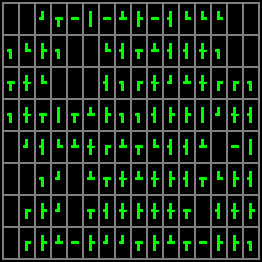
\includegraphics[scale=0.75]{SMT/pipe/shuffled.png}
\caption{Shuffled puzzle}
\end{figure}

\dots and solved:

\begin{figure}[H]
\label{fig:pipe_solved}
\centering
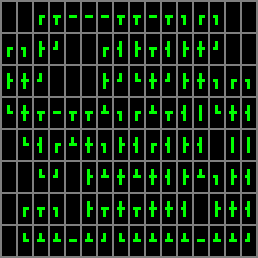
\includegraphics[scale=0.75]{SMT/pipe/solved.png}
\caption{Solved puzzle}
\end{figure}

Let's try to find a way to solve it.

\subsubsection{Generation}

First, we need to generate it.
Here is my quick idea on it.
Take 8*16 array of cells.
Each cell may contain some type of block.
There are joints between cells:

\pgfmathsetmacro\Width{16}
\pgfmathsetmacro\Height{8}
%\pgfmathsetmacro\Width{10}
%\pgfmathsetmacro\Height{5}
\pgfmathtruncatemacro\WidthMinusI{\Width - 1}
\pgfmathtruncatemacro\WidthMinusII{\Width - 2}
\pgfmathtruncatemacro\HeightMinusI{\Height - 1}
\pgfmathtruncatemacro\HeightMinusII{\Height - 2}
\pgfmathtruncatemacro\HeightPlusII{\Height + 2}
\pgfmathsetmacro\HeightPlusIi{\Height + 1.5}

% see also: http://www.texample.net/tikz/examples/euclid-algorithm/
\begin{center}
\begin{tikzpicture}[set style={{help lines}+=[dashed]},scale=0.7]

	\draw[style=help lines] (0,0) grid +(\Width,\Height);

	\foreach \c in {0,...,\WidthMinusI}
	{
		\foreach \r in {0,...,\HeightMinusII}
			\draw   [red,very thick,-] (\c+0.5,\r+0.75) -- (\c+0.5,\r+1.25);
		%\node[rotate=90] at (\c+0.5,\HeightPlusII) {\Large vjoints[\dots, \c] \normalsize};
		\node[rotate=90] at (\c+0.5,\HeightPlusII) {vjoints[\dots, \c]};
	}

	\foreach \r in {0,...,\HeightMinusI}
	{
		\foreach \c in {0,...,\WidthMinusII}
			\draw   [blue,very thick,-] (\c+0.75,\r+0.5) -- (\c+1.25,\r+0.5);
		\pgfmathtruncatemacro\hjointslabel{\HeightMinusI - \r}
		%\node at (-1.5,\r+0.5) {\large hjoints[\hjointslabel, \dots] \normalsize};
		\node at (-1.5,\r+0.5) {hjoints[\hjointslabel, \dots]};
	}

\end{tikzpicture}
\end{center}



Blue lines are horizontal joints, red lines are vertical joints.
We just set each joint to 0/false (absent) or 1/true (present), randomly.

Once set, it's now easy to find type for each cell.
There are:

\newcommand{\HeaderColor}{\cellcolor{blue!25}}
\begin{center}
\begin{longtable}{ | l | l | l | l | }
\hline
\HeaderColor joints & \HeaderColor our internal name & \HeaderColor angle & \HeaderColor symbol \\
\hline
0	&type 0		&	0$^{\circ}$	& (space)	\\
2	&type 2a	&	0$^{\circ}$	& \pmboxdrawuni{2503} \\ % ┃
2	&type 2a	&	90$^{\circ}$	& \pmboxdrawuni{2501} \\ % ━
2	&type 2b	&	0$^{\circ}$	& \pmboxdrawuni{250F} \\ % ┏
2	&type 2b	&	90$^{\circ}$	& \pmboxdrawuni{2513} \\ % ┓
2	&type 2b	&	180$^{\circ}$	& \pmboxdrawuni{251B} \\ % ┛
2	&type 2b	&	270$^{\circ}$	& \pmboxdrawuni{2517} \\ % ┗
3	&type 3		&	0$^{\circ}$	& \pmboxdrawuni{2523} \\ % ┣
3 	&type 3		&	90$^{\circ}$	& \pmboxdrawuni{2533} \\ % ┳
3	&type 3		&	180$^{\circ}$	& \pmboxdrawuni{252B} \\ % ┫
3	&type 3		&	270$^{\circ}$	& \pmboxdrawuni{253B} \\ % ┻
4	&type 4		&	0$^{\circ}$	& \pmboxdrawuni{254B} \\ % ╋
\hline
\end{longtable}
\end{center}

\textit{Dangling} joints can be preset at a first stage (i.e., cell with only one joint), but they are removed recursively,
these cells are transforming into empty cells.
Hence, at the end, all cells has at least two joints, and the whole plumbing system has no connections with outer
world---I hope this would make things clearer.

The C source code of generator is here: \url{https://github.com/DennisYurichev/SAT_SMT_article/tree/master/SMT/pipe/generator}.
All horizontal joints are stored in the global array \textit{hjoints[]} and vertical in \textit{vjoints[]}.

The C program generates ANSI-colored output like it has been showed above (\ref{fig:pipe_shuffled}, \ref{fig:pipe_solved}) plus
an array of types, with no angle information about each cell:

\begin{lstlisting}[label=init_cells]
[
["0", "0", "2b", "3", "2a", "2a", "2a", "3", "3", "2a", "3", "2b", "2b", "2b", "0", "0"],
["2b", "2b", "3", "2b", "0", "0", "2b", "3", "3", "3", "3", "3", "4", "2b", "0", "0"],
["3", "4", "2b", "0", "0", "0", "3", "2b", "2b", "4", "2b", "3", "4", "2b", "2b", "2b"],
["2b", "4", "3", "2a", "3", "3", "3", "2b", "2b", "3", "3", "3", "2a", "2b", "4", "3"],
["0", "2b", "3", "2b", "3", "4", "2b", "3", "3", "2b", "3", "3", "3", "0", "2a", "2a"],
["0", "0", "2b", "2b", "0", "3", "3", "4", "3", "4", "3", "3", "3", "2b", "3", "3"],
["0", "2b", "3", "2b", "0", "3", "3", "4", "3", "4", "4", "3", "0", "3", "4", "3"],
["0", "2b", "3", "3", "2a", "3", "2b", "2b", "3", "3", "3", "3", "2a", "3", "3", "2b"],
]
\end{lstlisting}

\subsubsection{Solving}

First of all, we would think about 8*16 array of cells, where each has four bits:
``T'' (top),
``B'' (bottom),
``L'' (left),
``R'' (right).
Each bit represents half of joint.

% see also: http://www.texample.net/tikz/examples/euclid-algorithm/
\begin{center}
\begin{tikzpicture}[set style={{help lines}+=[dashed]},scale=0.7]

	\draw[style=help lines] (0,0) grid +(\Width,\Height);
	
	\foreach \c in {0,...,\WidthMinusI}
		%\node[rotate=90] at (\c+0.5,\HeightPlusIi) {\Large [\dots, \c] \normalsize};
		\node[rotate=90] at (\c+0.5,\HeightPlusIi) {[\dots, \c]};
	
	\foreach \r in {0,...,\HeightMinusI}
	{
		\pgfmathtruncatemacro\hlabel{\HeightMinusI - \r}
		%\node at (-1.5,\r+0.5) {\large [\hlabel, \dots] \normalsize};
		\node at (-1.5,\r+0.5) {[\hlabel, \dots]};
	
		\pgfmathsetmacro\Shift{0.325}
		\foreach \c in {0,...,\WidthMinusI}
		{
			\node at (\c+0.5,\r+0.5 + \Shift) {\footnotesize T \normalsize};
			\node at (\c+0.5,\r+0.5 - \Shift) {\footnotesize B \normalsize};
			\node at (\c+0.5 - \Shift,\r+0.5) {\footnotesize L \normalsize};
			\node at (\c+0.5 + \Shift,\r+0.5) {\footnotesize R \normalsize};
		}
	}

\end{tikzpicture}
\end{center}


Now we define arrays of each of four half-joints + angle information:

\begin{lstlisting}
HEIGHT=8
WIDTH=16

# if T/B/R/L is Bool instead of Int, Z3 solver will work faster
T=[[Bool('cell_%d_%d_top' % (r, c)) for c in range(WIDTH)] for r in range(HEIGHT)]
B=[[Bool('cell_%d_%d_bottom' % (r, c)) for c in range(WIDTH)] for r in range(HEIGHT)]
R=[[Bool('cell_%d_%d_right' % (r, c)) for c in range(WIDTH)] for r in range(HEIGHT)]
L=[[Bool('cell_%d_%d_left' % (r, c)) for c in range(WIDTH)] for r in range(HEIGHT)]
A=[[Int('cell_%d_%d_angle' % (r, c)) for c in range(WIDTH)] for r in range(HEIGHT)]
\end{lstlisting}

We know that if each of half-joints is present, corresponding half-joint must be also present, and vice versa.
We define this using these constraints:

\begin{lstlisting}
# shorthand variables for True and False:
t=True
f=False

# "top" of each cell must be equal to "bottom" of the cell above
# "bottom" of each cell must be equal to "top" of the cell below
# "left" of each cell must be equal to "right" of the cell at left
# "right" of each cell must be equal to "left" of the cell at right
for r in range(HEIGHT):
    for c in range(WIDTH):
        if r!=0:
            s.add(T[r][c]==B[r-1][c])
        if r!=HEIGHT-1:
            s.add(B[r][c]==T[r+1][c])
        if c!=0:
            s.add(L[r][c]==R[r][c-1])
        if c!=WIDTH-1:
            s.add(R[r][c]==L[r][c+1])

# "left" of each cell of first column shouldn't have any connection
# so is "right" of each cell of the last column
for r in range(HEIGHT):
    s.add(L[r][0]==f)
    s.add(R[r][WIDTH-1]==f)

# "top" of each cell of the first row shouldn't have any connection
# so is "bottom" of each cell of the last row
for c in range(WIDTH):
    s.add(T[0][c]==f)
    s.add(B[HEIGHT-1][c]==f)
\end{lstlisting}

Now we'll enumerate all cells in the initial array (\ref{init_cells}).
First two cells are empty there. And the third one has type ``2b''.
This is ``\pmboxdrawuni{250F}'' % ┏
and it can be oriented in 4 possible ways.
And if it has angle 0$^{\circ}$, bottom and right half-joints are present, others are absent.
If it has angle 90$^{\circ}$, it looks like 
``\pmboxdrawuni{2513}'', % ┓
and bottom and left half-joints are present, others are absent.

In plain English: ``if cell of this type has angle 0$^{\circ}$, these half-joints must be present \textbf{OR}
if it has angle 90$^{\circ}$, these half-joints must be present, \textbf{OR}, etc, etc.''

Likewise, we define all these rules for all types and all possible angles:

\begin{lstlisting}
for r in range(HEIGHT):
    for c in range(WIDTH):
        ty=cells_type[r][c]

        if ty=="0":
            s.add(A[r][c]==f)
            s.add(T[r][c]==f, B[r][c]==f, L[r][c]==f, R[r][c]==f)

        if ty=="2a":
            s.add(Or(And(A[r][c]==0, L[r][c]==f, R[r][c]==f, T[r][c]==t, B[r][c]==t),   # §\pmboxdrawuni{2503}§
                    And(A[r][c]==90, L[r][c]==t, R[r][c]==t, T[r][c]==f, B[r][c]==f)))  # §\pmboxdrawuni{2501}§

        if ty=="2b":
            s.add(Or(And(A[r][c]==0, L[r][c]==f, R[r][c]==t, T[r][c]==f, B[r][c]==t),   # §\pmboxdrawuni{250F}§
                    And(A[r][c]==90, L[r][c]==t, R[r][c]==f, T[r][c]==f, B[r][c]==t),   # §\pmboxdrawuni{2513}§
                    And(A[r][c]==180, L[r][c]==t, R[r][c]==f, T[r][c]==t, B[r][c]==f),  # §\pmboxdrawuni{251B}§
                    And(A[r][c]==270, L[r][c]==f, R[r][c]==t, T[r][c]==t, B[r][c]==f))) # §\pmboxdrawuni{2517}§
	
        if ty=="3":
            s.add(Or(And(A[r][c]==0, L[r][c]==f, R[r][c]==t, T[r][c]==t, B[r][c]==t),   # §\pmboxdrawuni{2523}§
                    And(A[r][c]==90, L[r][c]==t, R[r][c]==t, T[r][c]==f, B[r][c]==t),   # §\pmboxdrawuni{2533}§
                    And(A[r][c]==180, L[r][c]==t, R[r][c]==f, T[r][c]==t, B[r][c]==t),  # §\pmboxdrawuni{252B}§
                    And(A[r][c]==270, L[r][c]==t, R[r][c]==t, T[r][c]==t, B[r][c]==f))) # §\pmboxdrawuni{253B}§

        if ty=="4":
            s.add(A[r][c]==0)
            s.add(T[r][c]==t, B[r][c]==t, L[r][c]==t, R[r][c]==t) # §\pmboxdrawuni{254B}§
\end{lstlisting}

Full source code is here: \url{https://github.com/DennisYurichev/SAT_SMT_article/blob/master/SMT/pipe/solver/solve_pipe_puzzle1.py}.

It produces this result (prints angle for each cell and (pseudo)graphical representation):

\begin{figure}[H]
\centering
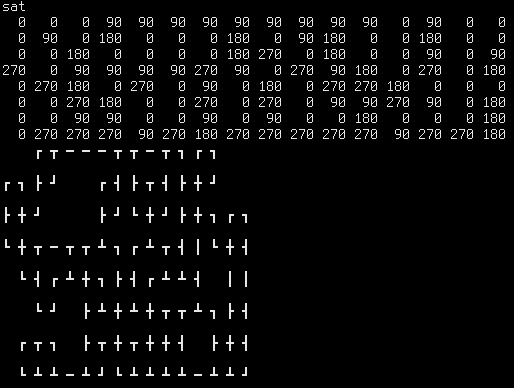
\includegraphics[scale=0.75]{SMT/pipe/solver/solver.png}
\caption{Solver script output}
\end{figure}

It worked $\approx 4$ seconds on my old and slow Intel Atom N455 1.66GHz.
Is it fast? I don't know, but again, what is really cool, we do not know about any mathematical background
of all this, we just defined cells, (half-)joints and defined relations between them.

Now the next question is, how many solutions are possible?
Using method described earlier (\ref{SMTEnumerate}), I've altered solver script
\footnote{\url{https://github.com/DennisYurichev/SAT_SMT_article/blob/master/SMT/pipe/solver/solve_pipe_puzzle2.py}} and solver
said two solutions are possible.

Let's compare these two solutions using gvimdiff:

\begin{figure}[H]
\centering
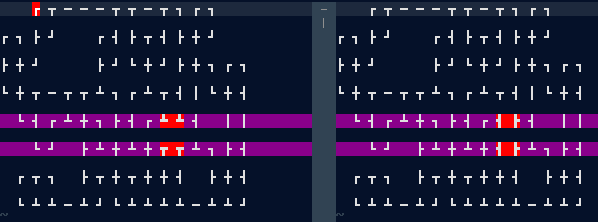
\includegraphics[scale=0.75]{SMT/pipe/solver/diff.png}
\caption{gvimdiff output (pardon my red cursor at left pane at left-top corner)}
\end{figure}

4 cells in the middle can be orientated differently.
Perhaps, other puzzles may produce different results.

P.S.
\textit{Half-joint} is defined as boolean type.
But in fact, the first version of the solver has been written using integer type for half-joints,
and 0 was used for False and 1 for True.
I did it so because I wanted to make source code tidier and narrower without using long words like ``False'' and ``True''.
And it worked, but slower. Perhaps, Z3 handles boolean data types faster? Better?
Anyway, I writing this to note that integer type can also be used instead of boolean, if needed.


\subsection{Recalculating micro-spreadsheet using Z3Py}

There is a nice exercise\footnote{Blog post in Russian: \url{http://thesz.livejournal.com/280784.html}}:
write a program to recalculate micro-spreadsheet, like this one:

\lstinputlisting{SMT/spreadsheet/test1}

As it turns out, though overkill, this can be solved using Z3 with little effort:

\lstinputlisting{SMT/spreadsheet/1.py}

( \url{https://github.com/DennisYurichev/yurichev.com/blob/master/blog/spreadsheet/1.py} )

All we do is just creating pack of variables for each cell, named A0, B1, etc, of integer type.
All of them are stored in \textit{cells[]} dictionary.
Key is a string.
Then we parse all the strings from cells, and add to list of constraints \textit{A0=123}
(in case of number in cell) or \textit{A0=B1+C2} (in case of expression in cell).
There is a slight preparation: string like \textit{A0+B2} becomes \textit{cells["A0"]+cells["B2"]}.

Then the string is evaluated using Python \textit{eval()} method,
which is highly dangerous
\footnote{\url{http://stackoverflow.com/questions/1832940/is-using-eval-in-python-a-bad-practice}}:
imagine if end-user could add a string to cell other than expression?
Nevertheless, it serves our purposes well, because this is a simplest way to pass a string with expression into Z3.

Z3 do the job with little effort:

\begin{lstlisting}
 % python 1.py test1
sat
1       0       135     82041
123     10      12      11
667     11      1342    83383
\end{lstlisting}

\subsubsection{Unsat core}

Now the problem: what if there is circular dependency? Like:

\lstinputlisting{SMT/spreadsheet/test_circular}

Two first cells of the last row (C0 and C1) are linked to each other.
Our program will just tells ``unsat'', meaning, it couldn't satisfy all constraints together.
We can't use this as error message reported to end-user, because it's highly unfriendly.

However, we can fetch \textit{unsat core}, i.e., list of variables which Z3 finds conflicting.

\begin{lstlisting}
...
s=Solver()
s.set(unsat_core=True)
...
        # add constraint:
        s.assert_and_track(e, coord_to_name(cur_R, cur_C))
...
if result=="sat":
...
else:
    print s.unsat_core()
\end{lstlisting}

( \url{https://github.com/DennisYurichev/yurichev.com/blob/master/blog/spreadsheet/2.py} )

We should explicitly turn on unsat core support and use \textit{assert\_and\_track()} instead of \textit{add()} method,
because this feature slows down the whole process, and is turned off by default.
That works:

\begin{lstlisting}
 % python 2.py test_circular
unsat
[C0, C1]
\end{lstlisting}

Perhaps, these variables could be removed from the 2D array, marked as \textit{unresolved}
and the whole spreadsheet could be recalculated again.

\subsubsection{Stress test}

How to generate large random spreadsheet?
What we can do.
First, create random \ac{DAG}, like this one:

\begin{figure}[H]
\centering
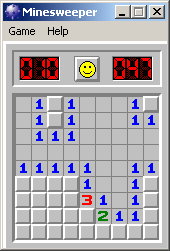
\includegraphics[width=\textwidth]{SMT/spreadsheet/1.png}
\caption{Random DAG}
\end{figure}

Arrows will represent information flow.
So a vertex (node) which has no incoming arrows to it (indegree=0), can be set to a random number.
Then we use topological sort to find dependencies between vertices.
Then we assign spreadsheet cell names to each vertex.
Then we generate random expression with random operations/numbers/cells to each cell,
with the use of information from topological sorted graph.

Wolfram Mathematica:

\begin{lstlisting}
(* Utility functions *)
In[1]:= findSublistBeforeElementByValue[lst_,element_]:=lst[[ 1;;Position[lst, element][[1]][[1]]-1]]

(* Input in 1..∞ range. 1->A0, 2->A1, etc *)
In[2]:= vertexToName[x_,width_]:=StringJoin[FromCharacterCode[ToCharacterCode["A"][[1]]+Floor[(x-1)/width]],ToString[Mod[(x-1),width]]]

In[3]:= randomNumberAsString[]:=ToString[RandomInteger[{1,1000}]]

In[4]:= interleaveListWithRandomNumbersAsStrings[lst_]:=Riffle[lst,Table[randomNumberAsString[],Length[lst]-1]]

(* We omit division operation because micro-spreadsheet evaluator can't handle division by zero *)
In[5]:= interleaveListWithRandomOperationsAsStrings[lst_]:=Riffle[lst,Table[RandomChoice[{"+","-","*"}],Length[lst]-1]]

In[6]:= randomNonNumberExpression[g_,vertex_]:=StringJoin[interleaveListWithRandomOperationsAsStrings[interleaveListWithRandomNumbersAsStrings[Map[vertexToName[#,WIDTH]&,pickRandomNonDependentVertices[g,vertex]]]]]

In[7]:= pickRandomNonDependentVertices[g_,vertex_]:=DeleteDuplicates[RandomChoice[findSublistBeforeElementByValue[TopologicalSort[g],vertex],RandomInteger[{1,5}]]]

In[8]:= assignNumberOrExpr[g_,vertex_]:=If[VertexInDegree[g,vertex]==0,randomNumberAsString[],randomNonNumberExpression[g,vertex]]

(* Main part *) 
(* Create random graph *)
In[21]:= WIDTH=7;HEIGHT=8;TOTAL=WIDTH*HEIGHT
Out[21]= 56

In[24]:= g=DirectedGraph[RandomGraph[BernoulliGraphDistribution[TOTAL,0.05]],"Acyclic"];

...

(* Generate random expressions and numbers *)
In[26]:= expressions=Map[assignNumberOrExpr[g,#]&,VertexList[g]];

(* Make 2D table of it *)
In[27]:= t=Partition[expressions,WIDTH];

(* Export as tab-separated values *)
In[28]:= Export["/home/dennis/1.txt",t,"TSV"]
Out[28]= /home/dennis/1.txt

In[29]:= Grid[t,Frame->All,Alignment->Left]
\end{lstlisting}

Here is an output from \textit{Grid[]}:

\begin{center}
\begin{tabular}{ | l | l | l | l | l | l | l |}
\hline
846 & 499 & A3*913-H4 & ... & ... & ... & ... \\
\hline
B4*860+D2 & 999 & 59 & ... & ... & ... & ... \\
\hline
G6*379-C3-436-C4-289+H6 & 972 & 804 & ... & ... & ... & ... \\
\hline
F2 & E0 & B6-731-D3+791+B4*92+C1 & ... & ... & ... & ... \\
\hline
519 & G1*402+D1*107*G3-458*A1 & D3 & ... & ... & ... & ... \\
\hline
F5-531+B5-222*E4 & 9 & B5+106*B6+600-B1 & ... & ... & ... & ... \\
\hline
C3-956*A5 & G4*408-D3*290*B6-899*G5+400+F1 & B2-701+H6 & ... & ... & ... & .. \\
\hline
B4-792*H4*407+F6-425-E1 & D2 & D3 & ... & ... & ... & ... \\
\hline
\end{tabular}
\end{center}



Using this script, I can generate random spreadsheet of $26 \cdot 500=13000$ cells,
which seems to be processed in couple of seconds.

\subsubsection{The files}

The files, including Mathematica notebook: \url{https://github.com/DennisYurichev/yurichev.com/tree/master/blog/spreadsheet}.


\subsection{Discrete tomography}

How computed tomography (CT scan) actually works?
A human body is bombarded by X-rays in various angles by X-ray tube in rotating torus.
X-ray detectors are also located in torus, and all the information is recorded.

Here is we can simulate simple tomograph.
An ``i'' character is rotating and will be ``enlighten'' at 4 angles.
Let's imagine, character is bombarded by X-ray tube at left.
All asterisks in each row is then summed and sum is "received" by X-ray detector at the right.

\begin{lstlisting}
WIDTH= 11 HEIGHT= 11
angle=(π/4)*0
    **      2
    **      2
            0
   ***      3
    **      2
    **      2
    **      2
    **      2
    **      2
   ****     4
            0
[2, 2, 0, 3, 2, 2, 2, 2, 2, 4, 0] ,
angle=(π/4)*1
            0
            0
  *         1
 **         2
    *       1
    **      2
     **     2
     ****   4
       *    1
      *     1
            0
[0, 0, 1, 2, 1, 2, 2, 4, 1, 1, 0] ,
angle=(π/4)*2
            0
            0
            0
            0
         *  1
** *******  9
** *******  9
   *     *  2
            0
            0
            0
[0, 0, 0, 0, 1, 9, 9, 2, 0, 0, 0] ,
angle=(π/4)*3
            0
            0
       *    1
       **   2
      ** *  3
     ***    3
    **      2
            0
  **        2
   *        1
            0
[0, 0, 1, 2, 3, 3, 2, 0, 2, 1, 0] ,
\end{lstlisting}

( The source code: \url{https://github.com/DennisYurichev/SAT_SMT_article/blob/master/SMT/tomo/gen.py} )

All we got from our toy-level tomograph is 4 vectors, these are sums of all asterisks in rows for 4 angles:

\begin{lstlisting}
[2, 2, 0, 3, 2, 2, 2, 2, 2, 4, 0] ,
[0, 0, 1, 2, 1, 2, 2, 4, 1, 1, 0] ,
[0, 0, 0, 0, 1, 9, 9, 2, 0, 0, 0] ,
[0, 0, 1, 2, 3, 3, 2, 0, 2, 1, 0] ,
\end{lstlisting}

How do we recover initial image?
We are going to represent 11*11 matrix, where sum of each row must be equal to some value we already know.
Then we rotate matrix, and do this again.

For the first matrix, the system of equations looks like that (we put there a values from the first vector):

\begin{lstlisting}
C1,1 + C1,2 + C1,3 + ... + C1,11 =      2
C2,1 + C2,2 + C2,3 + ... + C2,11 =      2

...

C10,1 + C10,2 + C10,3 + ... + C10,11 =  4
C11,1 + C11,2 + C11,3 + ... + C11,11 =  0
\end{lstlisting}

We also build similar systems of equations for each angle.

The ``rotate'' function has been taken from the generation program, because, due to Python's dynamic typization nature,
it's not important for the function to what operate on:
strings, characters, or Z3 variable instances, so it works very well for all of them.

\begin{lstlisting}
#-*- coding: utf-8 -*-

import math, sys
from z3 import *

# https://en.wikipedia.org/wiki/Rotation_matrix
def rotate(pic, angle):
    WIDTH=len(pic[0])
    HEIGHT=len(pic)
    #print WIDTH, HEIGHT
    assert WIDTH==HEIGHT
    ofs=WIDTH/2

    out = [[0 for x in range(WIDTH)] for y in range(HEIGHT)]

    for x in range(-ofs,ofs):
        for y in range(-ofs,ofs):
            newX = int(round(math.cos(angle)*x - math.sin(angle)*y,3))+ofs
            newY = int(round(math.sin(angle)*x + math.cos(angle)*y,3))+ofs
            # clip at boundaries, hence min(..., HEIGHT-1)
            out[min(newX,HEIGHT-1)][min(newY,WIDTH-1)]=pic[x+ofs][y+ofs]
    return out

vectors=[
[2, 2, 0, 3, 2, 2, 2, 2, 2, 4, 0] ,
[0, 0, 1, 2, 1, 2, 2, 4, 1, 1, 0] ,
[0, 0, 0, 0, 1, 9, 9, 2, 0, 0, 0] ,
[0, 0, 1, 2, 3, 3, 2, 0, 2, 1, 0]]

WIDTH = HEIGHT = len(vectors[0])

s=Solver()
cells=[[Int('cell_r=%d_c=%d' % (r,c)) for c in range(WIDTH)] for r in range(HEIGHT)]

# monochrome picture, only 0's or 1's:
for c in range(WIDTH):
    for r in range(HEIGHT):
        s.add(Or(cells[r][c]==0, cells[r][c]==1))

def all_zeroes_in_vector(vec):
    for v in vec:
        if v!=0:
            return False
    return True

ANGLES=len(vectors)
for a in range(ANGLES):
    angle=a*(math.pi/ANGLES)
    rows=rotate(cells, angle)
    r=0
    for row in rows:
        # skip empty rows:
        if all_zeroes_in_vector(row)==False:
            # sum of row must be equal to the corresponding element of vector:
            s.add(Sum(*row)==vectors[a][r])
        r=r+1

print s.check()
m=s.model()
for r in range(HEIGHT):
    for c in range(WIDTH):
        if str(m[cells[r][c]])=="1":
            sys.stdout.write("*")
        else:
            sys.stdout.write(" ")
    print ""
\end{lstlisting}

( The source code: \url{https://github.com/DennisYurichev/SAT_SMT_article/blob/master/SMT/tomo/solve.py} )

That works:

\begin{lstlisting}
% python solve.py
sat
    **
    **

   ***
    **
    **
    **
    **
    **
   ****
\end{lstlisting}

In other words, all SMT-solver does here is solving a system of equations.

So, 4 angles are enough.
What if we could use only 3 angles?

\begin{lstlisting}
WIDTH= 11 HEIGHT= 11
angle=(π/3)*0
    **      2
    **      2
            0
   ***      3
    **      2
    **      2
    **      2
    **      2
    **      2
   ****     4
            0
[2, 2, 0, 3, 2, 2, 2, 2, 2, 4, 0] ,
angle=(π/3)*1
            0
            0
            0
 **         2
 **         2
   ***      3
     ****   4
       **   2
       *    1
            0
            0
[0, 0, 0, 2, 2, 3, 4, 2, 1, 0, 0] ,
angle=(π/3)*2
            0
            0
            0
       **   2
       **   2
     *****  5
    **      2
 **         2
  *         1
            0
            0
[0, 0, 0, 2, 2, 5, 2, 2, 1, 0, 0] ,
\end{lstlisting}

No, it's not enough:

\begin{lstlisting}
% time python solve3.py
sat
 *  *
    **

     * **
   **
   *  *
    **
     *   *
*   *
   ****
\end{lstlisting}

However, the result is correct, but only 3 vectors allows too many possible ``initial images'',
and Z3 SMT-solver finds first.

Further reading:
\url{https://en.wikipedia.org/wiki/Discrete_tomography},
\url{https://en.wikipedia.org/wiki/2-satisfiability#Discrete_tomography}.


\subsection{Package manager and Z3}

Here is simplified example.
We have libA, libB, libC and libD, available in various versions (and flavors).
We're going to install programA and programB, which use these libraries.

\lstinputlisting{SMT/dep/dependency.py}

( The source code: \url{https://github.com/DennisYurichev/SAT_SMT_article/blob/master/SMT/dep/dependency.py} )

The output:

\begin{lstlisting}
sat
[libB = 5,
 libD = 999,
 libC = 10,
 programB = 7,
 programA = 1,
 libA = 2]
\end{lstlisting}

999 means that there is no need to install libD, it's not required by other packages.

Change version of ProgramB to v8 and it will says ``unsat'', meaning, there is a conflict:
ProgramA requires libA v2, but ProgramB v8 eventually requires newer libA.

Still, there is a work to do: ``unsat'' message is somewhat useless to end user,
some information about conflicting items should be printed.

Here is my another optimization problem example: \ref{set_cover}.

More about using SAT/SMT solvers in package managers: \url{https://research.swtch.com/version-sat},
\url{https://cseweb.ucsd.edu/~lerner/papers/opium.pdf}.

Now in the opposite direction: forcing aptitude package manager to solve Sudoku: \\
\url{http://web.archive.org/web/20160326062818/http://algebraicthunk.net/~dburrows/blog/entry/package-management-sudoku/}.

Some readers may ask, how to order libraries/programs/packages to be installed?
This is simpler problem, which is often solved by topological sorting.
The algorithm reorders graph in such a way so that vertices not depended on anything will be on the top of queue.
Next, there will be vertices dependend on vertices from the previous layer.
And so on.

\textit{make} UNIX utility does this while constructing order of items to be processed.
Even more: older \textit{make} utilities offloaded the job to the external utility (\textit{tsort}).
Some older UNIX has it, at least some versions of NetBSD
\footnote{\url{http://netbsd.gw.com/cgi-bin/man-cgi/man?tsort+1+NetBSD-current}}.


\subsection{Balanced Gray code and Z3 SMT solver}
\label{Gray_Z3}

Suppose, you are making a rotary encoder.
This is a device that can signal its angle in some form, like:

\begin{figure}[H]
\centering
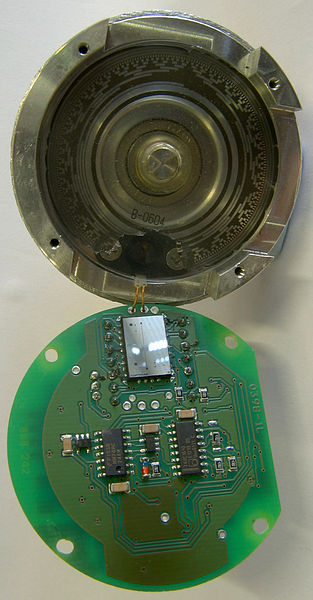
\includegraphics[scale=1]{SMT/gray/313px-Gray_code_rotary_encoder_13-track_opened.jpg}
\caption{Rotary encoder}
\end{figure}

( The image has been taken from Wikipedia: \url{https://en.wikipedia.org/wiki/Gray_code} )

% TODO FIX URL
Click on \href{https://raw.githubusercontent.com/DennisYurichev/yurichev.com/master/blog/gray/Gray_code_rotary_encoder_13-track_opened.jpg}{bigger image}.

This is a rotary (shaft) encoder: \url{https://en.wikipedia.org/wiki/Rotary_encoder}.

\begin{figure}[H]
\centering
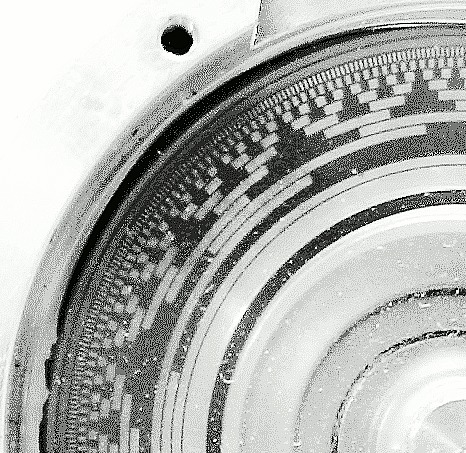
\includegraphics[scale=0.8]{SMT/gray/Rotary_Encoder_track_detail_scaled_crop.jpg}
\caption{Cropped and photoshopped version}
\end{figure}

( Source: \url{http://homepages.dordt.edu/~ddeboer//S10/304/c_at_d/304S10_RC_TRK.HTM} )

% TODO FIX URL
Click on
\href{https://raw.githubusercontent.com/DennisYurichev/yurichev.com/master/blog/gray/Rotary_Encoder_track_detail.jpg}{bigger one}.

There are pins and tracks on rotating wheel.
How would you do this?
Easiest way is to use binary code.
But it has a problem: when a wheel is rotating, in a moment of transition from one state to another, several bits may be changed, hence, undesirable state may be present for a short period of time.
This is bad.
To deal with it, Gray code was invented: only 1 bit is changed during rotation.
Like:

\begin{lstlisting}
Decimal Binary  Gray
0 	0000 	0000
1 	0001 	0001
2 	0010 	0011
3 	0011 	0010
4 	0100 	0110
5 	0101 	0111
6 	0110 	0101
7 	0111 	0100
8 	1000 	1100
9 	1001 	1101
10 	1010 	1111
11 	1011 	1110
12 	1100 	1010
13 	1101 	1011
14 	1110 	1001
15 	1111 	1000
\end{lstlisting}

Now the second problem. Look at the picture again. It has a lot of bit changes on the outer circles.
And this is electromechanical device.
Surely, you may want to make tracks as long as possible, to reduce wearing of both tracks and pins.
This is a first problem.
The second: wearing should be even across all tracks (this is balanced Gray code).

How we can find a table for all states using Z3:

\lstinputlisting{SMT/gray/gray.py}

% TODO FIX URL
( The source code: \url{https://github.com/DennisYurichev/yurichev.com/blob/master/blog/gray/gray.py} )

For 4 bits, 4 changes is enough:

\lstinputlisting{SMT/gray/4.txt}

% TODO FIX URL
8 changes for 5 bits: \url{https://github.com/DennisYurichev/yurichev.com/blob/master/blog/gray/5.txt}.
12 for 6 bits (or maybe even less): 
\url{https://github.com/DennisYurichev/yurichev.com/blob/master/blog/gray/6.txt}.

\subsubsection{Duke Nukem 3D from 1990s}

\begin{figure}[H]
\centering
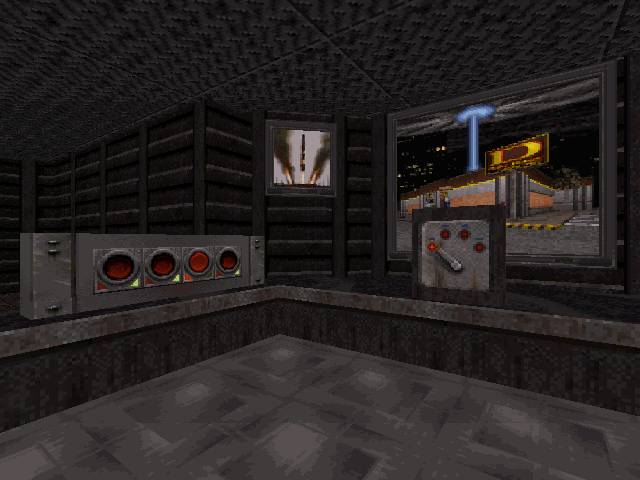
\includegraphics[scale=3]{SMT/gray/duke.png}
\caption{Duke Nukem 3D}
\end{figure}

Another application of Gray code:

\begin{lstlisting}
with.inspiring@flair.and.erudition (Mike Naylor) wrote:

>In Duke Nukem, you often come upon panels that have four buttons in a row,
>all in their "off" position. Each time you "push" a button, it toggles from
>one state to the other. The object is to find the unique combination that
>unlocks something in the game.

>My question is: What is the most efficient order in which to push the
>buttons so that every combination is tested with no wasted effort?

A Gray Code. :-)

(Oh, you wanted to know what one would be?  How about:
0000
0001
0011
0010
0110
0111
0101
0100
1100
1101
1111
1110
1010
1000
1001
1011

Or, if you prefer, with buttons A,B,C,D: D,C,D,B,D,C,D,A,D,C,D,B,C,D,C
It isn't the "canonical" Gray code (or if it is, it is by Divine
Providence), but it works.

Douglas Limmer -- lim...@math.orst.edu
"No wonder these mathematical wizards were nuts - went off the beam -
he'd be pure squirrel-food if he had half that stuff in _his_ skull!"
E. E. "Doc" Smith, _Second Stage Lensmen_
\end{lstlisting}

( \url{https://groups.google.com/forum/#!topic/rec.puzzles/Dh2H-pGJcbI} )

Obviously, using our solution, you can minimize all movements in this ancient videogame, for 4 switches, that would be 4*4=16 switches.
With our solution (balanced Gray code), wearing would be even across all 4 switches.

The same problem for MaxSAT: \ref{Gray_MaxSAT}.


\subsection{Tiling puzzle and Z3 SMT solver}
\label{tiling_Z3}

This is classic problem: given 12 polyomino titles, cover mutilated chessboard with them (it has 60 squares with no central 4 squares).

The problem is covered at least in \href{https://arxiv.org/pdf/cs/0011047.pdf}{Donald E. Knuth - Dancing Links},
and this Z3 solution has been inspired by it.

Another thing I've added: graph coloring. You see, my script gives correct solutions, but somewhat unpleasant visually.
So I used colored pseudographics. There are 12 tiles, it's not a problem to assign 12 colors to them.
But there is another heavily used SAT problem: graph coloring.

Given a graph, assign a color to each vertex/node, so that colors wouldn't be equal in adjacent nodes.
The problem can be solved easily in SMT: assign variable to each vertex.
If two vertices are connected, add a constraint: \textit{vertex1\_color != vertex2\_color}.
As simple as that.
In my case, each polynomio is vertex and if polyomino is adjacent to another polyomino, an edge/link is added between vertices.
So I did, and output is now colored.

But this is planar graph (i.e., a graph which is, if represented in two-dimensional space has no intersected edges/links).
And here is a famous four color theorem can be used.
The solution of tiled polynomios is in fact like planar graph, or, a map, like a world map.
Theorem states that any planar graph (or map) can be colored only 4 colors.

This is true, even more, several tilings can be colors with only 3 colors:

\begin{figure}[H]
\centering
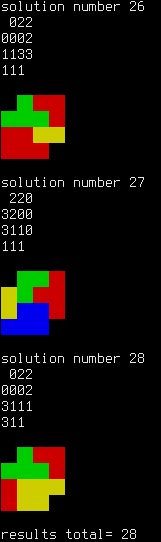
\includegraphics[scale=1]{SMT/tiling/small.png}
\caption{}
\end{figure}

Now the classic: 12 pentominos and "mutilated" chess board, several solutions:

% TODO side by side in table:
\begin{figure}[H]
\centering
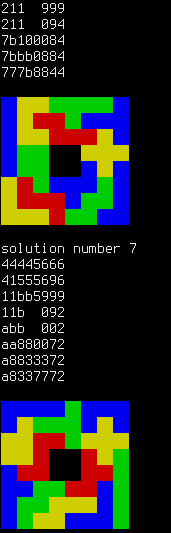
\includegraphics[scale=1]{SMT/tiling/big1.png}
\caption{}
\end{figure}

\begin{figure}[H]
\centering
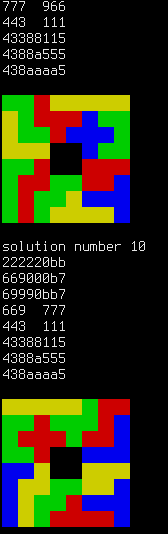
\includegraphics[scale=1]{SMT/tiling/big2.png}
\caption{}
\end{figure}

% FIXME URL
The source code: \url{.../tiling.py}.

Further reading: \url{https://en.wikipedia.org/wiki/Exact_cover#Pentomino_tiling}.

Four-color theorem has an interesting story, it has been finally proved in 2005 by Coq proof assistant:
\url{https://en.wikipedia.org/wiki/Four_color_theorem}.


\subsection{Solving pocket Rubik’s cube (2*2*2) using Z3}
\label{PocketCubeSMT}

\begin{figure}[H]
\centering
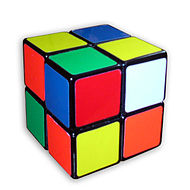
\includegraphics[scale=0.75]{SMT/rubik2/failed/190px-Pocket_cube_scrambled.jpg}
\caption{Pocket cube}
\end{figure}

( The image has been taken \href{https://en.wikipedia.org/wiki/Pocket_Cube}{from Wikipedia}. )

Solving Rubik's cube is not a problem, finding shortest solution is.

\subsubsection{Intro}

First, a bit of terminology.
There are 6 colors we have: white, green, blue, orange, red, yellow.
We also have 6 sides: front, up, down, left, right, back.

This is how we will name all facelets:

% TODO TikZ
\begin{lstlisting}
        U1 U2
        U3 U4

       -------
L1 L2 | F1 F2 | R1 R2 | B1 B2
L3 L4 | F3 F4 | R3 R4 | B3 B4
       -------

        D1 D2
        D3 D4
\end{lstlisting}

Colors on a solved cube are:

\begin{lstlisting}
    G G
    G G
    ---
R R|W W|O O|Y Y
R R|W W|O O|Y Y
    ---
    B B
    B B
\end{lstlisting}

There are 6 possible turns: front, left, right, back, up, down.
But each turn can be clockwise, counterclockwise and half-turn (equal to two CW or two CCW).
Each CW is equal to 3 CCW and vice versa.
Hence, there are 6*3=18 possible turns.

It is known, that 11 turns (including half-turns) are enough to solve any pocket cube
(\href{https://en.wikipedia.org/wiki/Optimal_solutions_for_Rubik%27s_Cube}{God’s algorithm}).
This means, \href{http://mathworld.wolfram.com/GraphDiameter.html}{graph has a diameter} of 11.
For 3*3*3 cube one need 20 turns (\url{http://www.cube20.org/}).
See also: \url{https://en.wikipedia.org/wiki/Rubik%27s_Cube_group}.

\subsubsection{Z3}

There are 6 sides and 4 facelets on each, hence, 6*4=24 variables we need to define a state.

Then we define how state is transformed after each possible turn:

\begin{lstlisting}
FACE_F, FACE_U, FACE_D, FACE_R, FACE_L, FACE_B = 0,1,2,3,4,5

def rotate_FCW(s):
    return [
        [ s[FACE_F][2], s[FACE_F][0], s[FACE_F][3], s[FACE_F][1] ],   # for F
        [ s[FACE_U][0], s[FACE_U][1], s[FACE_L][3], s[FACE_L][1] ],   # for U
        [ s[FACE_R][2], s[FACE_R][0], s[FACE_D][2], s[FACE_D][3] ],   # for D
        [ s[FACE_U][2], s[FACE_R][1], s[FACE_U][3], s[FACE_R][3] ],   # for R
        [ s[FACE_L][0], s[FACE_D][0], s[FACE_L][2], s[FACE_D][1] ],   # for L
        [ s[FACE_B][0], s[FACE_B][1], s[FACE_B][2], s[FACE_B][3] ] ]  # for B

def rotate_FH(s):
    return [
        [ s[FACE_F][3], s[FACE_F][2], s[FACE_F][1], s[FACE_F][0] ],
        [ s[FACE_U][0], s[FACE_U][1], s[FACE_D][1], s[FACE_D][0] ],
        [ s[FACE_U][3], s[FACE_U][2], s[FACE_D][2], s[FACE_D][3] ],
        [ s[FACE_L][3], s[FACE_R][1], s[FACE_L][1], s[FACE_R][3] ],
        [ s[FACE_L][0], s[FACE_R][2], s[FACE_L][2], s[FACE_R][0] ],
        [ s[FACE_B][0], s[FACE_B][1], s[FACE_B][2], s[FACE_B][3] ] ]

...
\end{lstlisting}

Then we define a function, which takes turn number and transforms a state:

\begin{lstlisting}
# op is turn number
def rotate(turn, state, face, facelet):
    return If(op==0,  rotate_FCW (state)[face][facelet],
           If(op==1,  rotate_FCCW(state)[face][facelet],
           If(op==2,  rotate_UCW (state)[face][facelet],
           If(op==3,  rotate_UCCW(state)[face][facelet],
           If(op==4,  rotate_DCW (state)[face][facelet],

...

           If(op==17, rotate_BH  (state)[face][facelet],
                      0))))))))))))))))))
\end{lstlisting}

Now set "solved" state, initial state and connect everything:

\begin{lstlisting}
move_names=["FCW", "FCCW", "UCW", "UCCW", "DCW", "DCCW", "RCW", "RCCW", "LCW", "LCCW", "BCW", "BCCW", "FH", "UH", "DH", "RH", "LH", "BH"]

def colors_to_array_of_ints(s):
    return [{"W":0, "G":1, "B":2, "O":3, "R":4, "Y":5}[c] for c in s]

def set_current_state (d):
    F=colors_to_array_of_ints(d["FACE_F"])
    U=colors_to_array_of_ints(d["FACE_U"])
    D=colors_to_array_of_ints(d["FACE_D"])
    R=colors_to_array_of_ints(d["FACE_R"])
    L=colors_to_array_of_ints(d["FACE_L"])
    B=colors_to_array_of_ints(d["FACE_B"])
    return F,U,D,R,L,B # return tuple

# 4
init_F, init_U, init_D, init_R, init_L, init_B=set_current_state({"FACE_F":"RYOG", "FACE_U":"YRGO", "FACE_D":"WRBO", "FACE_R":"GYWB", "FACE_L":"BYWG", "FACE_B":"BOWR"})

...

for TURNS in range(1,12): # 1..11
    print "turns=", TURNS

    s=Solver()

    state=[[[Int('state%d_%d_%d' % (n, side, i)) for i in range(FACELETS)] for side in range(FACES)] for n in range(TURNS+1)]
    op=[Int('op%d' % n) for n in range(TURNS+1)]

    for i in range(FACELETS):
        s.add(state[0][FACE_F][i]==init_F[i])
        s.add(state[0][FACE_U][i]==init_U[i])
        s.add(state[0][FACE_D][i]==init_D[i])
        s.add(state[0][FACE_R][i]==init_R[i])
        s.add(state[0][FACE_L][i]==init_L[i])
        s.add(state[0][FACE_B][i]==init_B[i])

    # solved state
    for face in range(FACES):
        for facelet in range(FACELETS):
            s.add(state[TURNS][face][facelet]==face)

    # turns:
    for turn in range(TURNS):
        for face in range(FACES):
            for facelet in range(FACELETS):
                s.add(state[turn+1][face][facelet]==rotate(op[turn], state[turn], face, facelet))

    if s.check()==sat:
        print "sat"
        m=s.model()
        for turn in range(TURNS):
            print move_names[int(str(m[op[turn]]))]
        exit(0)
\end{lstlisting}

% FIXME URL
( The full source code: \url{https://github.com/DennisYurichev/yurichev.com/blob/master/blog/rubik/rubik2_z3.py} )

That works:

\begin{lstlisting}
turns= 1
turns= 2
turns= 3
turns= 4
sat
RCW
UCW
DCW
RCW
\end{lstlisting}

...but very slow. It takes up to 1 hours to find a path of 8 turns, which is not enough, we need 11.

Nevetheless, I decided to include Z3 solver as a demonstration.

See also: solving pocket cube using SAT solver: \ref{PocketCubeSAT}.


\subsection{Rubik’s cube (3*3*3) and Z3 SMT-solver}

As I wrote before, I couldn't solve even 2*2*2 pocket cube with Z3 (\ref{PocketCubeSMT}),
but I wanted to play with it further, and found
that it's still possible to solve one face instead of all 6.

I tried to model color of each facelet using integer sort (type), but now I can use bool: white facelet is True and all other non-white is False.
I can encode state of Rubik's cube like that: "W" for white facelet, "." for other.

Now the process of solving is a matter of minutes on a decent computer, or faster.

\begin{lstlisting}
#!/usr/bin/env python

from z3 import *

FACES=6
FACELETS=9

def rotate_FCW(s):
        return [
                [ s[0][6], s[0][3], s[0][0], s[0][7], s[0][4], s[0][1], s[0][8], s[0][5], s[0][2], ],  # new F
                [ s[1][0], s[1][1], s[1][2], s[1][3], s[1][4], s[1][5], s[4][8], s[4][5], s[4][2], ],  # new U
                [ s[3][6], s[3][3], s[3][0], s[2][3], s[2][4], s[2][5], s[2][6], s[2][7], s[2][8], ],  # new D
                [ s[1][6], s[3][1], s[3][2], s[1][7], s[3][4], s[3][5], s[1][8], s[3][7], s[3][8], ],  # new R
                [ s[4][0], s[4][1], s[2][0], s[4][3], s[4][4], s[2][1], s[4][6], s[4][7], s[2][2], ],  # new L
                [ s[5][0], s[5][1], s[5][2], s[5][3], s[5][4], s[5][5], s[5][6], s[5][7], s[5][8], ] ] # new B

def rotate_FH(s):
        return [
                [ s[0][8], s[0][7], s[0][6], s[0][5], s[0][4], s[0][3], s[0][2], s[0][1], s[0][0], ],
                [ s[1][0], s[1][1], s[1][2], s[1][3], s[1][4], s[1][5], s[2][2], s[2][1], s[2][0], ],
                [ s[1][8], s[1][7], s[1][6], s[2][3], s[2][4], s[2][5], s[2][6], s[2][7], s[2][8], ],
                [ s[4][8], s[3][1], s[3][2], s[4][5], s[3][4], s[3][5], s[4][2], s[3][7], s[3][8], ],
                [ s[4][0], s[4][1], s[3][6], s[4][3], s[4][4], s[3][3], s[4][6], s[4][7], s[3][0], ],
                [ s[5][0], s[5][1], s[5][2], s[5][3], s[5][4], s[5][5], s[5][6], s[5][7], s[5][8], ] ]


...


def rotate(op, st, side, j):
	return If(op==0, rotate_FCW(st)[side][j],
		If(op==1, rotate_FCCW(st)[side][j],
		If(op==2, rotate_UCW(st)[side][j],
		If(op==3, rotate_UCCW(st)[side][j],
		If(op==4, rotate_DCW(st)[side][j],
		If(op==5, rotate_DCCW(st)[side][j],
		If(op==6, rotate_RCW(st)[side][j],
		If(op==7, rotate_RCCW(st)[side][j],
		If(op==8, rotate_LCW(st)[side][j],
		If(op==9, rotate_LCCW(st)[side][j],
		If(op==10, rotate_BCW(st)[side][j],
		If(op==11, rotate_BCCW(st)[side][j],
		If(op==12, rotate_FH(st)[side][j],
		If(op==13, rotate_UH(st)[side][j],
		If(op==14, rotate_DH(st)[side][j],
		If(op==15, rotate_RH(st)[side][j],
		If(op==16, rotate_LH(st)[side][j],
		If(op==17, rotate_BH(st)[side][j],
			rotate_BH(st)[side][j], # default
			))))))))))))))))))

move_names=["FCW", "FCCW", "UCW", "UCCW", "DCW", "DCCW", "RCW", "RCCW", "LCW", "LCCW", "BCW", "BCCW", "FH", "UH", "DH", "RH", "LH", "BH"]

def colors_to_array_of_ints(s):
    rt=[]
    for c in s:
	if c=='W':
            rt.append(True)
        else:
            rt.append(False)
    return rt

def set_current_state (d):
    F=colors_to_array_of_ints(d["F"])
    U=colors_to_array_of_ints(d["U"])
    D=colors_to_array_of_ints(d["D"])
    R=colors_to_array_of_ints(d["R"])
    L=colors_to_array_of_ints(d["L"])
    B=colors_to_array_of_ints(d["B"])
    return F,U,D,R,L,B # return tuple

init_F, init_U, init_D, init_R, init_L, init_B=set_current_state({"F":"....W..W.", "U":"...W...W.", "D":".......W.", "R":"..W...W..", "L":"......W..", "B":"..W......"})

for STEPS in range(1, 20):
	print "trying %d steps" % STEPS

	s=Solver()
	state=[[[Bool('state%d_%d_%d' % (n, side, i)) for i in range(FACELETS)] for side in range(FACES)] for n in range(STEPS+1)]

	op=[Int('op%d' % n) for n in range(STEPS+1)]

	# initial state
	for i in range(FACELETS):
		s.add(state[0][0][i]==init_F[i])
		s.add(state[0][1][i]==init_U[i])
		s.add(state[0][2][i]==init_D[i])
		s.add(state[0][3][i]==init_R[i])
		s.add(state[0][4][i]==init_L[i])
		s.add(state[0][5][i]==init_B[i])

	# "must be" state for one (front/white) face
	for j in range(FACELETS):
		s.add(state[STEPS][0][j]==True)

	for n in range(STEPS):
		for side in range(FACES):
			for j in range(FACELETS):
				s.add(state[n+1][side][j]==rotate(op[n], state[n], side, j))

	if s.check()==sat:
		print "sat"
		m=s.model()
		for n in range(STEPS):
			print move_names[int(str(m[op[n]]))]
		exit(0)
\end{lstlisting}

% FIXME URL
( The full source code: \url{...} )

Now the fun statistics.
Using random walk I collected 928 states and then I tried to solve one (white/front) face for each state.

\begin{lstlisting}
      1 turns= 4
      5 turns= 5
     57 turns= 6
    307 turns= 7
    501 turns= 8
     56 turns= 9
      1 turns= 10
\end{lstlisting}

It seems that majority of all states can be solved for 7-8 half turns (half-turn is one of 18 turns we used here).
But there is at least one state which must be solved with 10 half turns.
Maybe 10 is a "\href{http://www.cube20.org/}{god’s number}" for one face, like 20 for all 6 faces?


\subsection{Cribbage}

I've found this problem in [Ronald L. Graham, Donald E. Knuth, Oren Patashnik -- Concrete Mathematics]:

\begin{framed}
\begin{quotation}
Cribbage players have long been aware that 15 = 7 + 8 = 4 + 5 + 6 =
1 + 2 + 3 + 4 + 5 . Find the number of ways to represent 1050 as a sum of
consecutive positive integers. (The trivial representation `1050' by itself
counts as one way; thus there are four, not three, ways to represent 15
as a sum of consecutive positive integers. Incidentally, a knowledge of
cribbage rules is of no use in this problem.)
\end{quotation}
\end{framed}

My solution:

\lstinputlisting{SMT/cribbage.py}

The result:

\begin{lstlisting}
(3 terms) 349 + ... + 351 == 1050
(4 terms) 261 + ... + 264 == 1050
(5 terms) 208 + ... + 212 == 1050
(7 terms) 147 + ... + 153 == 1050
(12 terms) 82 + ... + 93 == 1050
(15 terms) 63 + ... + 77 == 1050
(20 terms) 43 + ... + 62 == 1050
(21 terms) 40 + ... + 60 == 1050
(25 terms) 30 + ... + 54 == 1050
(28 terms) 24 + ... + 51 == 1050
(35 terms) 13 + ... + 47 == 1050
\end{lstlisting}


\subsection{Ménage problem}

\begin{lstlisting}
In combinatorial mathematics, the ménage problem or problème des ménages[1] asks for the number of different ways in which it is possible to seat a set of male-female couples at a dining table so that men and women alternate and nobody sits next to his or her partner. This problem was formulated in 1891 by Édouard Lucas and independently, a few years earlier, by Peter Guthrie Tait in connection with knot theory.[2] For a number of couples equal to 3, 4, 5, ...  the number of seating arrangements is

    12, 96, 3120, 115200, 5836320, 382072320, 31488549120, ... (sequence A059375 in the OEIS). 
\end{lstlisting}

( \href{https://en.wikipedia.org/wiki/M%C3%A9nage_problem}{Wikipedia}. )

We can count it using Z3, but also get actual men/women allocations:

\lstinputlisting{SMT/menage.py}

( \url{URL} )

For 3 couples:

\begin{lstlisting}
  men 0 2 1
women  1 0 2

  men 1 2 0
women  0 1 2

  men 0 1 2
women  2 0 1

  men 2 1 0
women  0 2 1

  men 2 0 1
women  1 2 0

  men 1 0 2
women  2 1 0

results total= 6
however, according to https://oeis.org/A059375 : 12
\end{lstlisting}

We are getting ``half'' of results because men and women can be then swapped (their sex swapped (or reassigned))
and you've got another 6 results.
6+6=12 in total.
This is kind of symmetry.

For 4 couples:

\begin{lstlisting}

...

  men 3 0 2 1
women  1 3 0 2

  men 3 0 1 2
women  2 3 0 1

  men 1 0 2 3
women  3 1 0 2

  men 2 0 1 3
women  3 2 0 1

results total= 48
however, according to https://oeis.org/A059375 : 96
\end{lstlisting}

For 5 couples:

\begin{lstlisting}

...

  men 0 4 1 2 3
women  1 3 0 4 2

  men 0 3 1 2 4
women  1 4 0 3 2

  men 0 3 1 2 4
women  1 0 4 3 2

  men 4 3 1 0 2
women  0 2 4 1 3

results total= 1560
however, according to https://oeis.org/A059375 : 3120
\end{lstlisting}


\subsection{Stable marriage problem}

See also in
\href{https://en.wikipedia.org/wiki/Stable_marriage_problem}{Wikipedia} and 
\href{https://rosettacode.org/wiki/Stable_marriage_problem}{Rosetta code}.

Layman's explanation in Russian: \url{https://lenta.ru/articles/2012/10/15/nobel/}.

My solution is much less efficient, because much simpler/better algorithm exists (Gale/Shapley algorithm),
but I did it to demonstrate the essence of the problem plus as a yet another SMT-solvers and Z3 demonstration.

See comments:

\lstinputlisting{SMT/stable_marriage/stable.py}

( The source code: \url{URL/stable.py} )

Result is seems to be correct:

\begin{lstlisting}
sat

ManChoice:
abe <-> ivy
bob <-> cath
col <-> dee
dan <-> fay
ed <-> jan
fred <-> bea
gav <-> gay
hal <-> eve
ian <-> hope
jon <-> abi

WomanChoice:
abi <-> jon
bea <-> fred
cath <-> bob
dee <-> col
eve <-> hal
fay <-> dan
gay <-> gav
hope <-> ian
ivy <-> abe
jan <-> ed
\end{lstlisting}

This is what we did in plain English language.
``Connect men and women somehow, we don't care how.
But no pair must exist of those who prefer each other (simultaneously) over their current spouses''.
Gale/Shapley algorithm uses ``steps'' to ``stabilize'' marriage.
There are no ``steps'', all pairs are married couples already.

Another important thing to notice: only one solution must exist.

\begin{lstlisting}
...

results=[]

# enumerate all possible solutions:
while True:
    if s.check() == sat:
        m = s.model()
        #print m
        results.append(m)
        block = []
        for d in m:
            c=d()
            block.append(c != m[d])
        s.add(Or(block))
    else:
        print "results total=", len(results)
        break

...
\end{lstlisting}

( The source code: \url{URL/stable2.py} )

That reports only 1 model available, which is correct indeed.


\subsection{Enumerating all possible inputs for a specific regular expression}

Regular expression if first converted to \ac{FSM} before matching.
Hence, many \ac{RE} libraries has two functions: ``compile'' and ``execute''
(when you match many strings against single RE, no need to recompile it to \ac{FSM} each time).

And I've found this website, which can visualize FSM (finite state machine) for a regular expression.
\url{http://hokein.github.io/Automata.js/}.
This is fun!

This \ac{FSM} (\ac{DFA}) is for the expression \TT{(dark|light)?(red|blue|green)(ish)?}

\begin{figure}[H]
\centering
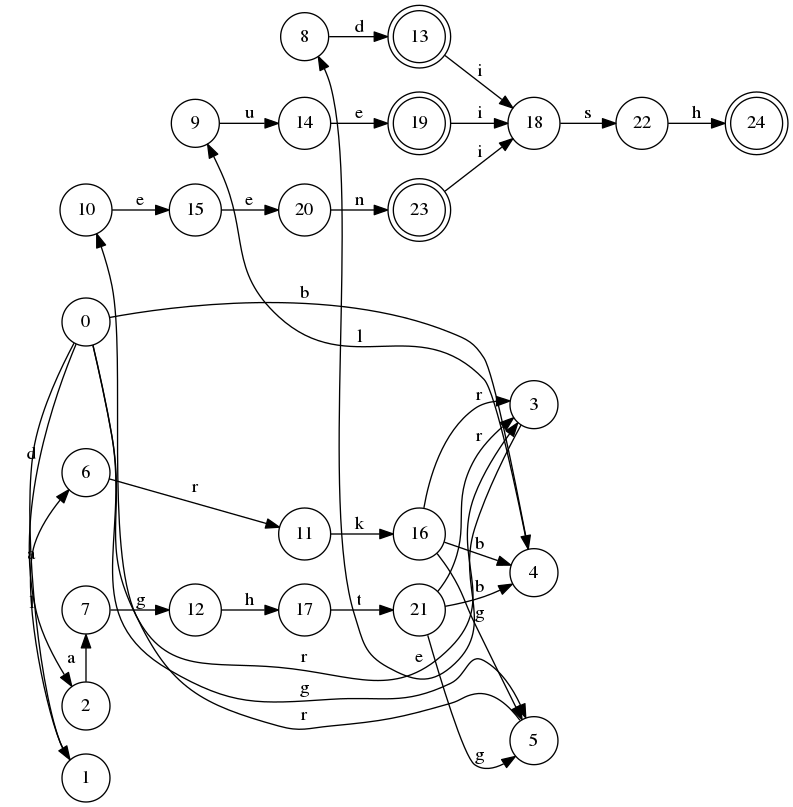
\includegraphics[scale=0.6]{SMT/regexp/1.png}
\caption{}
\end{figure}

% FSM.png
Another version: URL.

Accepting states are in double circles, these are the states where matching process stops.

How can we generate an input string which regular expression would match?
In other words, which inputs \ac{FSM} would accept?
This task is surprisingly simple for SMT-solver.

We just define a transition function.
For each pair (state, input) it defines new state.

\ac{FSM} has been visualized by the website mentioned above, and I used this information to write ``transition()'' function.

Then we chain transition functions... then we try a chain for all lengths in range of 2..14.

\lstinputlisting{SMT/regexp/re.py}

Results:

\lstinputlisting{SMT/regexp/res.txt}

As simple as this.

% TODO \gls
It can be said, what we did is enumeration of all paths between two vertices of a digraph (representing \ac{FSM}).

Also, the ``transition()'' function itself can act as a RE matcher, with no relevance to SMT solver(s).
Just feed input characters to it and track state.
Whenever you hit one of accepting states, return ``match'', whenever you hit \TT{INVALID\_STATE}, return ``no match''.


\subsection{Dependency graphs and topological sorting}

Topological sorting is an operation many programmers well familiar with: this is what ``make'' tool
do when it find an order of items to process.
Items not dependent of anything can be processed first.
The most dependent items at the end.

Dependency graph is a graph and topological sorting is such a ``contortion'' of the a graph,
when you can see an order of items.

For example, let's create a sample graph in Wolfram Mathematica:

\begin{lstlisting}
In[]:= g = Graph[{7 -> 1, 7 -> 0, 5 -> 1, 3 -> 0, 3 -> 4, 1 -> 2, 1 -> 6, 
   1 -> 4, 0 -> 6}, VertexLabels -> "Name"]
\end{lstlisting}

\begin{figure}[H]
\centering
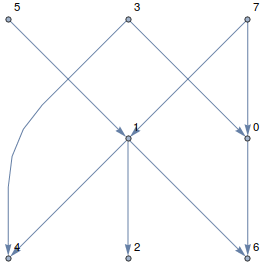
\includegraphics[scale=0.6]{SMT/tsort/math.png}
\caption{}
\end{figure}

Each arrow shows that an item is needed by an item arrow pointing to, i.e., if ``a -> b'', then item ``a'' must be first
processed, because ``b'' needs it, or ``b'' depends on ``a''.

How Mathematica would ``sort'' the dependency graph?

\begin{lstlisting}
In[]:= TopologicalSort[g]
Out[]= {7, 3, 0, 5, 1, 4, 6, 2}
\end{lstlisting}

So you're going to process item 7, then 3, 0, and 2 at the very end.

\href{https://en.wikipedia.org/wiki/Topological_sorting}{The algorithm in the Wikipedia article}
is probably used in the ``make'' and whatever IDE you use for building your code.

Also, many UNIX platforms had separate ``tsort'' utility:
\url{https://en.wikipedia.org/wiki/Tsort}.

How would ``tsort'' sort the graph? I'm making the text file with input data:

\begin{lstlisting}
7 1
7 0
5 1
3 0
3 4
1 2
1 6
1 4
0 6
\end{lstlisting}

And run tsort:

\begin{lstlisting}
 % tsort tst
3
5
7
0
1
4
6
2
\end{lstlisting}

Now I'll use Z3 SMT-solver for topological sort, which is overkill, but quite spectacular: all we need to do
is to add constraint for each edge (or ``connection'') in graph, if ``a -> b'', then ``a'' must be less then ``b'', where
each variable reflects ordering.

\lstinputlisting{SMT/tsort/tsort.py}

Almost the same result, but also correct:

\begin{lstlisting}
sat
[3, 5, 7, 0, 1, 2, 4, 6]
\end{lstlisting}


\subsection{Travelling salesman problem}

This is it:

\lstinputlisting{SMT/TSP/TSP.py}

The result:

\begin{lstlisting}
sat
Dallas (1240 mi to the next city) ->
Los Angeles (831 mi to the next city) ->
Denver (700 mi to the next city) ->
Minneapolis (355 mi to the next city) ->
Chicago (713 mi to the next city) ->
New York (1374 mi to the next city) ->
distance_total= 5213 mi
\end{lstlisting}

Map I generated with Wolfram Mathematica:

\begin{figure}[H]
\centering
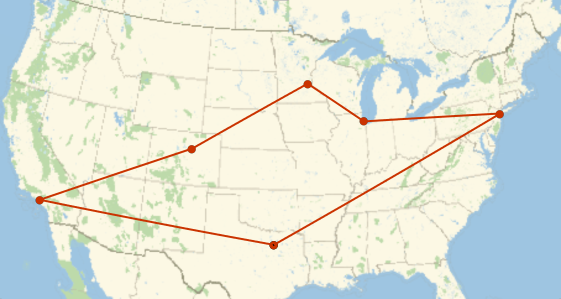
\includegraphics[scale=0.6]{SMT/TSP/map1.png}
\caption{}
\end{figure}

Maximizing:

\begin{lstlisting}
sat
Dallas (862 mi to the next city) ->
Minneapolis (700 mi to the next city) ->
Denver (1631 mi to the next city) ->
New York (2451 mi to the next city) ->
Los Angeles (1745 mi to the next city) ->
Chicago (803 mi to the next city) ->
distance_total= 8192 mi
\end{lstlisting}

The map:

\begin{figure}[H]
\centering
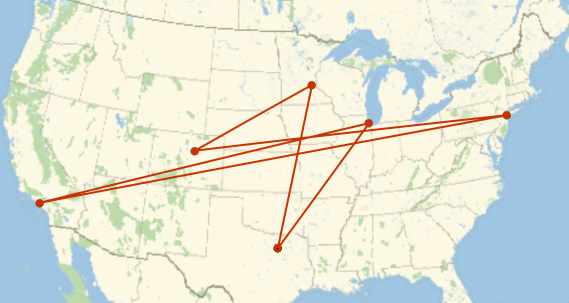
\includegraphics[scale=0.6]{SMT/TSP/map2.png}
\caption{}
\end{figure}

I could only process 6 cities, and it takes starting at several seconds up to 1 minute on my venerable Intel Quad-Core Xeon E3-1220 3.10GHz.
Perhaps, this is not a right tool for the job, well-known TSP algorithms way faster.

Even bruteforce enumeration is way faster ($6!=720$ paths).

However, it still can serve as demonstration.


\subsection{Crossword generator}

We assign an integer to each character in crossword, it reflects ASCII code of it.

Then we enumerate all possible horizontal/vertical ``sticks'' longer than 1 and assign words to them.

For example, there is a horizontal stick of length 3.
And we have such 3-letter words in our dictionary: ``the'', ``she'', ``xor''.

We add the following constraint:

\begin{lstlisting}
Or(
	And(chars[X][Y]=='t', chars[X][Y+1]=='h', chars[X][Y+2]=='e'),
	And(chars[X][Y]=='s', chars[X][Y+1]=='h', chars[X][Y+2]=='e'),
	And(chars[X][Y]=='x', chars[X][Y+1]=='o', chars[X][Y+2]=='r'))
\end{lstlisting}

One of these words would be choosen automatically.

Index of each word is also considered, because duplicates are not allowed.

Sample pattern:

\begin{lstlisting}
**** **********
 * * *  * * * *
***************
 * * *  * * * *
********* *****
 * * * * * *  *
****** ********
   * * * * *   
******** ******
*  * * * * * * 
***** *********
* * * *  * * * 
***************
* * * *  * * * 
********** ****
\end{lstlisting}

Sample result:

\begin{lstlisting}
spur stimulated
 r e c  i a h e
congratulations
 m u t  a i s c
violation niece
 s a e p e n  n
rector penitent
   i i o c e
accounts herald
s  n g e a r o
press edinburgh
e x e n  t p i
characteristics
t c l r  n e a
satisfying dull

horizontal:
((0, 0), (0, 3)) spur
((0, 5), (0, 14)) stimulated
((2, 0), (2, 14)) congratulations
((4, 0), (4, 8)) violation
((4, 10), (4, 14)) niece
((6, 0), (6, 5)) rector
((6, 7), (6, 14)) penitent
((8, 0), (8, 7)) accounts
((8, 9), (8, 14)) herald
((10, 0), (10, 4)) press
((10, 6), (10, 14)) edinburgh
((12, 0), (12, 14)) characteristics
((14, 0), (14, 9)) satisfying
((14, 11), (14, 14)) dull
vertical:
((8, 0), (14, 0)) aspects
((0, 1), (6, 1)) promise
((10, 2), (14, 2)) exact
((0, 3), (10, 3)) regulations
((10, 4), (14, 4)) seals
((0, 5), (9, 5)) scattering
((10, 6), (14, 6)) entry
((4, 7), (10, 7)) opposed
((0, 8), (4, 8)) milan
((5, 9), (14, 9)) enchanting
((0, 10), (4, 10)) latin
((4, 11), (14, 11)) interrupted
((0, 12), (4, 12)) those
((8, 13), (14, 13)) logical
((0, 14), (6, 14)) descent
\end{lstlisting}

Unsat is possible if the dictionary is too small or have no words of length present in pattern.

The source code:

\lstinputlisting{SMT/cross/cross_Z3.py}

The files, including my dictionary: \url{https://github.com/DennisYurichev/yurichev.com...}.


\subsection{Exercise 15 from TAOCP ``7.1.3 Bitwise tricks and techniques''}

Page 53 from the fasc1a.ps, or: \url{http://www.cs.utsa.edu/~wagner/knuth/fasc1a.pdf}

\begin{figure}[H]
\label{fig:pipe_shuffled}
\centering
\frame{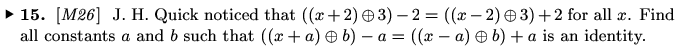
\includegraphics[scale=0.6]{SMT/TAOCP_7_1_3_exercise_15/page53.png}}
\caption{Page 53}
\end{figure}

Soltuion:

\begin{lstlisting}
from z3 import *

s=Solver()

a, b=BitVecs('a b', 4)
x, y=BitVecs('x y', 4)

s.add(ForAll(x, ForAll(y,  ((x+a)^b)-a == ((x-a)^b)+a  )))

# enumerate all possible solutions:
results=[]
while True:
    if s.check() == sat:
        m = s.model()
        print m

        results.append(m)
        block = []
        for d in m:
            c=d()
            block.append(c != m[d])
        s.add(Or(block))
    else:
        print "results total=", len(results)
        break
\end{lstlisting}

For 4-bit bitvectors:

\begin{lstlisting}

...

[b = 7, a = 0]
[b = 6, a = 8]
[b = 7, a = 8]
[b = 6, a = 12]
[b = 7, a = 12]
[b = 12, a = 0]
[b = 13, a = 0]
[b = 12, a = 8]
[b = 13, a = 8]
[b = 12, a = 4]
[b = 13, a = 4]
[b = 12, a = 12]
[b = 13, a = 12]
[b = 14, a = 0]
[b = 15, a = 0]
[b = 14, a = 4]
[b = 15, a = 4]
[b = 14, a = 8]
[b = 15, a = 8]
[b = 14, a = 12]
[b = 15, a = 12]
results total= 128
\end{lstlisting}


\subsection{Anroid lock screen (9 dots) has 140240 possible ways to (un)lock it}

How would you count?

\begin{lstlisting}
from z3 import *

"""
1 2 3
4 5 6
7 8 9
"""

# where the next dot can be if the current dot is at $a$
# next dot can only be a neighbour
# here we define starlike connections between dots (as in Android lock screen)
# this is like switch() or multiplexer

# lines like these are also counted:
# * . .
# . . *
# . * .
def next_dot(a, b):
    return If(a==1, Or(b==2, b==4, b==5, b==6, b==8),
        If(a==2, Or(b==1, b==3, b==4, b==5, b==6, b==7, b==9),
        If(a==3, Or(b==2, b==5, b==6, b==4, b==8),
        If(a==4, Or(b==1, b==2, b==5, b==7, b==8, b==3, b==9),
        If(a==5, Or(b==1, b==2, b==3, b==4, b==6, b==7, b==8, b==9),
        If(a==6, Or(b==2, b==3, b==5, b==8, b==9, b==1, b==7),
        If(a==7, Or(b==4, b==5, b==8, b==2, b==6),
        If(a==8, Or(b==4, b==5, b==6, b==7, b==9, b==1, b==3),
        If(a==9, Or(b==5, b==6, b==8, b==4, b==2),
            False))))))))) # default

# if only non-diagonal lines between dots are allowed:
"""
def next_dot(a, b):
    return If(a==1, Or(b==2, b==4),
        If(a==2, Or(b==1, b==3, b==5),
        If(a==3, Or(b==2, b==6),
        If(a==4, Or(b==1, b==5, b==7),
        If(a==5, Or(b==2, b==4, b==6, b==8),
        If(a==6, Or(b==3, b==5, b==9),
        If(a==7, Or(b==4, b==8),
        If(a==8, Or(b==5, b==7, b==9),
        If(a==9, Or(b==6, b==8),
            False))))))))) # default
"""

# old version, hasn't counted lines like
# * . .
# . . *
# . * .

"""
def next_dot(a, b):
    return If(a==1, Or(b==2, b==4, b==5),
        If(a==2, Or(b==1, b==3, b==4, b==5, b==6),
        If(a==3, Or(b==2, b==5, b==6),
        If(a==4, Or(b==1, b==2, b==5, b==7, b==8),
        If(a==5, Or(b==1, b==2, b==3, b==4, b==6, b==7, b==8, b==9),
        If(a==6, Or(b==2, b==3, b==5, b==8, b==9),
        If(a==7, Or(b==4, b==5, b==8),
        If(a==8, Or(b==4, b==5, b==6, b==7, b==9),
        If(a==9, Or(b==5, b==6, b==8),
            False))))))))) # default
"""

def paths_for_length (LENGTH):
    s=Solver()

    path=[Int('path_%d' % i) for i in range(LENGTH)]

    # all elements of path must be distinct
    s.add(Distinct(path))

    # all elements in [1..9] range:
    for i in range(LENGTH):
        s.add(And(path[i]>=1, path[i]<=9))

    # next element of path is defined by next_dot() function, unless it's the last one:
    for i in range(LENGTH-1):
        s.add(next_dot(path[i], path[i+1]))

    results=[]

    # enumerate all possible solutions:
    while True:
        if s.check() == sat:
            m = s.model()
            tmp=[]
            for i in range(LENGTH):
                tmp.append(m[path[i]].as_long())
            #print m
            print "path", tmp
            # print visual representation:
            for k in [[1,2,3],[4,5,6],[7,8,9]]:
                for j in k:
                    if j in tmp:
                        print tmp.index(j)+1,
                    else:
                        print ".",
                print ""
            print ""
            results.append(m)
            block = []
            for d in m:
                c=d()
                block.append(c != m[d])
            s.add(Or(block))
        else:
            print "length=", LENGTH, "results total=", len(results)
            return len(results)

total=0
for l in range(2,10):
    total=total+paths_for_length(l)

print "total=", total
\end{lstlisting}

Sample paths of 7 elements:

\begin{lstlisting}
...

path [7, 5, 1, 4, 8, 6, 3]
3 . 7
4 2 6
1 5 .

path [9, 5, 7, 4, 8, 6, 3]
. . 7
4 2 6
3 5 1

path [9, 5, 1, 4, 8, 6, 3]
3 . 7
4 2 6
. 5 1

...
\end{lstlisting}

Each element of ``path'' is number of dot, like on phone's keypad:

\begin{lstlisting}
1 2 3
4 5 6
7 8 9
\end{lstlisting}

Numbers on $3 \cdot 3$ box represent a sequence: which dot is the 1st, 2nd, etc...

Of 9:

\begin{lstlisting}
...

path [7, 8, 9, 5, 4, 1, 2, 6, 3]
6 7 9
5 4 8
1 2 3

path [1, 4, 7, 5, 2, 3, 6, 9, 8]
1 5 6
2 4 7
3 9 8

path [9, 6, 8, 7, 4, 1, 5, 2, 3]
6 8 9
5 7 2
4 3 1

...
\end{lstlisting}

All possible paths: \url{FIXME/all.bz2}

Statistics:

\begin{lstlisting}
length= 2 results total= 56
length= 3 results total= 304
length= 4 results total= 1400
length= 5 results total= 5328
length= 6 results total= 16032
length= 7 results total= 35328
length= 8 results total= 49536
length= 9 results total= 32256
total= 140240
\end{lstlisting}

What if only non-diagonal lines would be allowed (which isn't a case of a real Android lock screen)?

\begin{lstlisting}
length= 2 results total= 24
length= 3 results total= 44
length= 4 results total= 80
length= 5 results total= 104
length= 6 results total= 128
length= 7 results total= 112
length= 8 results total= 112
length= 9 results total= 40
total= 644
\end{lstlisting}

Also, at first, when I published this note, lines like these weren't counted (but allowable on Andoird lock screen, as it was pointed out by @mztropics):

\begin{lstlisting}
* . .
. . *
. * .
\end{lstlisting}

And the [incorrect] statistics was like this:

\begin{lstlisting}
length= 2 results total= 40
length= 3 results total= 160
length= 4 results total= 496
length= 5 results total= 1208
length= 6 results total= 2240
length= 7 results total= 2984
length= 8 results total= 2384
length= 9 results total= 784
total= 10296
\end{lstlisting}

Now you can see, how drastically number of all possibilities can change, when you add $\approx 2$ more branches at each element of path.


\subsection{Recreational math, calculator's keypad and divisibility}

I've once read about this puzzle.
Imagine calculator's keypad:

\begin{lstlisting}
789
456
123
\end{lstlisting}

If you form any rectangle or square out of keys, like:

\begin{lstlisting}
 7 8 9
+---+
|4 5|6
|1 2|3
+---+
\end{lstlisting}

The number is 4521. Or 2145, or 5214.
All these numbers are divisible by 11, 111 and 111.
One explanation: \url{https://files.eric.ed.gov/fulltext/EJ891796.pdf}.

However, I could try to prove that all these numbers are indeed divisible.

\begin{lstlisting}[style=custompy]

from z3 import *

"""
We will keep track on numbers using row/col representation:

 |0 1 2 <-col
-|- - -
0|7 8 9
1|4 5 6
2|1 2 3
^
|
row

"""

# map coordinates to number on keypad:
def coords_to_num (r, c):
    return If(And(r==0, c==0), 7,
    If(And(r==0, c==1), 8,
    If(And(r==0, c==2), 9,
    If(And(r==1, c==0), 4,
    If(And(r==1, c==1), 5,
    If(And(r==1, c==2), 6,
    If(And(r==2, c==0), 1,
    If(And(r==2, c==1), 2,
    If(And(r==2, c==2), 3, 9999)))))))))

s=Solver()

# coordinates of upper left corner:
from_r, from_c = Ints('from_r from_c')
# coordinates of bottom right corner:
to_r, to_c = Ints('to_r to_c')

# all coordinates are in [0..2]:
s.add(And(from_r>=0, from_r<=2, from_c>=0, from_c<=2))
s.add(And(to_r>=0, to_r<=2, to_c>=0, to_c<=2))

# bottom-right corner is always under left-upper corner, or equal to it, or to the right of it:
s.add(to_r>=from_r)
s.add(to_c>=from_c)

# numbers on keypads for all 4 corners:
LT, RT, BL, BR = Ints('LT RT BL BR')

# ... which are:
s.add(LT==coords_to_num(from_r, from_c))
s.add(RT==coords_to_num(from_r, to_c))
s.add(BL==coords_to_num(to_r, from_c))
s.add(BR==coords_to_num(to_r, to_c))

# 4 possible 4-digit numbers formed by passing by 4 corners:
n1, n2, n3, n4 = Ints('n1 n2 n3 n4')

s.add(n1==LT*1000 + RT*100 + BR*10 + BL)
s.add(n2==RT*1000 + BR*100 + BL*10 + LT)
s.add(n3==BR*1000 + BL*100 + LT*10 + RT)
s.add(n4==BL*1000 + LT*100 + RT*10 + BR)

# what we're going to do?
prove=False
enumerate_rectangles=True

assert prove != enumerate_rectangles

if prove:
    # prove by finding counterexample.
    # find any variable state for which remainder will be non-zero:
    s.add(And((n1%11) != 0), (n1%111) != 0, (n1%1111) != 0)
    s.add(And((n2%11) != 0), (n2%111) != 0, (n2%1111) != 0)
    s.add(And((n3%11) != 0), (n3%111) != 0, (n3%1111) != 0)
    s.add(And((n4%11) != 0), (n4%111) != 0, (n4%1111) != 0)

    # this is impossible, we're getting unsat here, because no counterexample exist:
    print s.check()

# ... or ...

if enumerate_rectangles:
    # enumerate all possible solutions:
    results=[]
    while True:
        if s.check() == sat:
            m = s.model()
            #print_model(m)
            print m
            print m[n1]
            print m[n2]
            print m[n3]
            print m[n4]
            results.append(m)
            block = []
            for d in m:
                c=d()
                block.append(c != m[d])
            s.add(Or(block))
        else:
            print "results total=", len(results)
            break

\end{lstlisting}

Enumeration. only 36 rectangles exist on 3*3 keypad:

\begin{lstlisting}
[n1 = 7821,
 BL = 1,
 n2 = 8217,
 to_r = 2,
 LT = 7,
 RT = 8,
 BR = 2,
 n4 = 1782,
 from_r = 0,
 n3 = 2178,
 from_c = 0,
 to_c = 1]
7821
8217
2178
1782
[n1 = 7931,
 BL = 1,
 n2 = 9317,
 to_r = 2,
 LT = 7,
 RT = 9,
 BR = 3,
 n4 = 1793,
 from_r = 0,
 n3 = 3179,
 from_c = 0,
 to_c = 2]
7931
9317
3179
1793

...

[n1 = 5522,
 BL = 2,
 n2 = 5225,
 to_r = 2,
 LT = 5,
 RT = 5,
 BR = 2,
 n4 = 2552,
 from_r = 1,
 n3 = 2255,
 from_c = 1,
 to_c = 1]
5522
5225
2255
2552
results total= 36
\end{lstlisting}


\subsection{Knight's tour}

\lstinputlisting[style=custompy]{SMT/knight_tour/knight_tour_Z3.py}

Can find a closed knight's tour on 8*8 chess board for 150s on Intel Quad-Core Xeon E3-1220 3.10GHz:

\begin{lstlisting}
 0 57 44 41  2 39 12 29
43 46  1 58 11 30 23 38
56 63 42 45 40  3 28 13
47  8 59 10 31 24 37 22
60 55 62 51  4 27 14 25
 7 48  9 32 17 34 21 36
54 61 50  5 52 19 26 15
49  6 53 18 33 16 35 20
\end{lstlisting}

However, this is WAY slower than C implementation on Rosetta Code: \url{https://rosettacode.org/wiki/Knight%27s_tour#C}
... which uses Warnsdorf's rule: \url{https://en.wikipedia.org/wiki/Knight%27s_tour#Warnsdorff.27s_algorithm}.

Another program for Z3 for finding Hamiltonian cycle: \url{https://github.com/Z3Prover/z3/blob/master/examples/python/hamiltonian/hamiltonian.py}.
(Clever trick of using remainder.)


\subsection{Hilbert's 10th problem, Fermat’s last theorem and SMT solvers}

Hilbert's 10th problem states that you cannot devise an algorithm which can solve any diophantine equation over integers.
However, it's important to understand, that this is possible over fixed-size bitvectors.

Fermat's last theorem states that there are no integer solution(s) for $a^n + b^n = c^n$, for $n>=3$.

Let's prove it for n=3 and for a in 0..255 range:

\lstinputlisting[style=custompy]{SMT/Hilbert_10/fermat.py}

Z3 gives "unsat", meaning, it couldn't find any a/b/c.
However, this is possible to check even using brute-force search.

If to replace "BitVecs" by "Ints", Z3 would give "unknown":

\lstinputlisting[style=custompy]{SMT/Hilbert_10/fermat2.py}

In short: anything is decidable (you can build an algorithm which can solve equation or not) under fixed-size bitvectors.
Given enough computational power, you can solve such equations for big bit-vectors.
But this is not possible for integers or bit-vectors of any size.

Another interesting reading about this by Leonardo de Moura:
\url{https://stackoverflow.com/questions/13898175/how-does-z3-handle-non-linear-integer-arithmetic}.



\subsection{List of SMT-solvers}

\begin{itemize}

\item Yices\footnote{\url{http://yices.csl.sri.com/}}, created by Bruno Dutertre et al.

\item Z3\footnote{\url{https://github.com/Z3Prover/z3}},
created by Leonardo de Moura, Nikolaj Bjorner, Christoph M. Wintersteiger.

	Many examples here uses Python 3.x API for Z3.
	Here is how to install it in Ubuntu:

	\begin{lstlisting}
	sudo apt-get install python3-pip
	sudo pip3 install z3-solver
	\end{lstlisting}

\item STP\footnote{\url{https://github.com/stp/stp}}, used in KLEE.

\item CVC3/CVC4\footnote{\url{http://cvc4.stanford.edu/}}.

\item Boolector\footnote{\url{http://fmv.jku.at/boolector/}}, created by Aina Niemetz, Mathias Preiner and Armin Biere.

\item Alt-Ergo\footnote{\url{https://alt-ergo.ocamlpro.com/}}, used in Frama-C.

\item MathSAT\footnote{\url{http://mathsat.fbk.eu/}}. Created by Alberto Griggio, Alessandro Cimatti and Roberto Sebastiani.

\item veriT\footnote{\url{http://www.verit-solver.org/}}.
Created by David Déharbe, Pascal Fontaine, Haniel Barbosa.
Bitvectors are not supported.

\item MK85\footnote{\url{https://github.com/DennisYurichev/MK85}}. Created by Dennis Yurichev, as a toy-level bit-blaster.

\end{itemize}



